% Options for packages loaded elsewhere
\PassOptionsToPackage{unicode}{hyperref}
\PassOptionsToPackage{hyphens}{url}
%
\documentclass[
  table]{report}
\usepackage{amsmath,amssymb}
\usepackage{iftex}
\ifPDFTeX
  \usepackage[T1]{fontenc}
  \usepackage[utf8]{inputenc}
  \usepackage{textcomp} % provide euro and other symbols
\else % if luatex or xetex
  \usepackage{unicode-math} % this also loads fontspec
  \defaultfontfeatures{Scale=MatchLowercase}
  \defaultfontfeatures[\rmfamily]{Ligatures=TeX,Scale=1}
\fi
\usepackage{lmodern}
\ifPDFTeX\else
  % xetex/luatex font selection
\fi
% Use upquote if available, for straight quotes in verbatim environments
\IfFileExists{upquote.sty}{\usepackage{upquote}}{}
\IfFileExists{microtype.sty}{% use microtype if available
  \usepackage[]{microtype}
  \UseMicrotypeSet[protrusion]{basicmath} % disable protrusion for tt fonts
}{}
\makeatletter
\@ifundefined{KOMAClassName}{% if non-KOMA class
  \IfFileExists{parskip.sty}{%
    \usepackage{parskip}
  }{% else
    \setlength{\parindent}{0pt}
    \setlength{\parskip}{6pt plus 2pt minus 1pt}}
}{% if KOMA class
  \KOMAoptions{parskip=half}}
\makeatother
\usepackage{xcolor}
\usepackage{graphicx}
\makeatletter
\def\maxwidth{\ifdim\Gin@nat@width>\linewidth\linewidth\else\Gin@nat@width\fi}
\def\maxheight{\ifdim\Gin@nat@height>\textheight\textheight\else\Gin@nat@height\fi}
\makeatother
% Scale images if necessary, so that they will not overflow the page
% margins by default, and it is still possible to overwrite the defaults
% using explicit options in \includegraphics[width, height, ...]{}
\setkeys{Gin}{width=\maxwidth,height=\maxheight,keepaspectratio}
% Set default figure placement to htbp
\makeatletter
\def\fps@figure{htbp}
\makeatother
\setlength{\emergencystretch}{3em} % prevent overfull lines
\providecommand{\tightlist}{%
  \setlength{\itemsep}{0pt}\setlength{\parskip}{0pt}}
\setcounter{secnumdepth}{5}
\AtBeginDocument{\let\maketitle\relax}
\usepackage{lastpage} % Calculate the last page of the document
\usepackage{tocbibind} % Insert custom table of content items
\usepackage{graphicx} % import figure
\usepackage{float} % Allow for more granular control of float of figures
\usepackage{setspace}
\usepackage{lipsum} % Generate lorem ipsum text
\usepackage{acronym}
\usepackage[fontsize=12pt]{scrextend}
\usepackage{fontspec} % change to system font
\usepackage{tcolorbox} % Fancy text boxes that are pretty
\tcbset{ definitionstyle/.style={ colback=orange!5!white, colframe=orange!80!black, top=0.25cm, bottom=0.25cm, before=\vspace{0.5cm}, after=\vspace{0.5cm} } }
\usepackage{todonotes}
\usepackage[style=apa, natbib=true]{biblatex}
\addbibresource{nebula.bib}
\addbibresource{manual-nebula.bib}
\DefineBibliographyExtras{english}{}
\usepackage{csquotes}
\usepackage{hyperref}
\usepackage{cleveref}
\usepackage{booktabs}
\usepackage{array}
\onehalfspacing
\usepackage[a4paper,width=150mm,top=25mm,bottom=25mm]{geometry}
\usepackage{fancyhdr}
\pagestyle{fancy}
\fancyhf{}
\fancyfoot[C]{}
\usepackage[bottom]{footmisc}
\tcbuselibrary{theorems}
\renewcommand{\headrulewidth}{0pt}
\renewcommand{\arraystretch}{1.7} % Adjust the value as needed
\usepackage{epigraph}
\setlength\epigraphwidth{.6\textwidth}
\setmainfont{Georgia}
\usepackage{titlesec}
\newfontfamily\headingfont{Avenir}
\titleformat{\chapter}[display]{\headingfont\large}{\chaptertitlename\ \thechapter}{20pt}{\Huge}
\titleformat*{\section}{\Large\headingfont}
\titleformat*{\subsection}{\large\headingfont}
\titleformat*{\subsubsection}{\large\headingfont}
\hyphenation{Web-Assembly}
\usepackage{booktabs}
\usepackage{longtable}
\usepackage{array}
\usepackage{multirow}
\usepackage{wrapfig}
\usepackage{float}
\usepackage{colortbl}
\usepackage{pdflscape}
\usepackage{tabu}
\usepackage{threeparttable}
\usepackage{threeparttablex}
\usepackage[normalem]{ulem}
\usepackage{makecell}
\usepackage{xcolor}
\ifLuaTeX
  \usepackage{selnolig}  % disable illegal ligatures
\fi
\usepackage[]{biblatex}
\usepackage{bookmark}
\IfFileExists{xurl.sty}{\usepackage{xurl}}{} % add URL line breaks if available
\urlstyle{same}
\hypersetup{
  pdftitle={Nebula},
  pdfauthor={Marius Nilsen Kluften},
  hidelinks,
  pdfcreator={LaTeX via pandoc}}

\title{Nebula}
\usepackage{etoolbox}
\makeatletter
\providecommand{\subtitle}[1]{% add subtitle to \maketitle
  \apptocmd{\@title}{\par {\large #1 \par}}{}{}
}
\makeatother
\subtitle{Comparing two waves of cloud computing}
\author{Marius Nilsen Kluften}
\date{2024}

\begin{document}
\maketitle

\begin{titlepage}
\thispagestyle{fancy}
\fancyfoot[C]{2024}
\centering
{\Huge\bfseries Nebula\par}

\vspace{0.5cm}

{\Huge\itshape Comparing two waves of cloud compute\par}

\vspace{1cm}

{\Large Marius Nilsen Kluften\par}

\vspace{1cm}


\includegraphics[width=0.4\textwidth]{assets/uio-logo.png}\\[1cm]

{\Large Thesis submitted for the degree of\par}
{\Large Master in Informatics: Programming and System Architecture\par}

\vspace{0.25cm}

{\Large 60 credits\par}

\vspace{1cm}

{\Large Institute of Informatics\par}

{\Large Faculty of mathematics and natural sciences\par}

{\Large University of Oslo\par}

\end{titlepage}

\newpage

\begin{center}
\vspace*{\fill} 
\Huge \textbf{Nebula} \\[10pt]
\vspace{2cm} 
\Large \textit{Comparing two waves of cloud compute} \\[20pt]
\vspace{2cm} 
\Large Marius Nilsen Kluften \\[30pt]
\vspace*{\fill} 
\end{center}

\newpage
\listoftodos
\newpage

\null\vfill
\begin{flushleft}
\Large © 2024 Marius Nilsen Kluften\par
\Large Nebula \par
\Large https://duo.uio.no/ \par
\Large Printed: Reprosentralen, University of Oslo \par
\end{flushleft}

\newpage
\fancyfoot[C]{ \thepage\ }
\pagenumbering{roman}

\vspace*{\fill}
\begin{center}
\begin{minipage}{0.75\textwidth}

\addcontentsline{toc}{chapter}{Abstract}
\chapter*{Abstract}

The ever increasing demand for cloud services has resulted in the expansion of
energy-intensive data centers, the ICT industry accounts for about 1 \% of global 
electricity use, highlighting a need for sustainable options
in cloud computing architectures.

\vspace{0.25cm}

This thesis investigates WebAssembly, a technology originally intended for running 
in the browser, as a potential contender in the space of technologies to
consider in cloud native applications. Leveraging the inherent efficiency,
portability and lower startup times of WebAssembly modules, this thesis presents an
approach that aligns with green energy principles, while maintaining performance and
scalability, essential for cloud services. 

\vspace{0.25cm}

Preliminary findings suggest that programs compiled to WebAssembly modules have 
reduced startup and runtimes, which hopefully leads to less energy
consumption and offering a viable pathway towards a more sustainable cloud.

\end{minipage}
\end{center}
\vspace*{\fill}

\newpage

\vspace*{\fill}
\begin{center}
\begin{minipage}{0.75\textwidth}

\addcontentsline{toc}{chapter}{Acknowledgements}
\chapter*{Acknowledgments}


The idea for the topic for this thesis appeared in an episode of the podcast
"Rustacean station". Matt Butcher, the CEO of Fermyon, told the story of his
journey through the different waves of cloud computing, and why Fermyon 
decided to bet on WebAssembly for the next big wave of cloud compute.

\vspace{0.25cm}

The capabilities of WebAssembly running on the server, with the aid of
the WebAssembly System Interface project, caught my interest and started 
the snowball that ended up as the avalanche that is this thesis. 

\vspace{0.25cm}

I'd like to thank Matt Butcher and the people over at Fermyon for inadvertently 
inspiring my topic. 

\vspace{0.25cm}

Furthermore I'd like to thank my two supervisors Joachim Tilsted Kristensen and 
Michael Kirkedal Thomsen, whom I somehow managed to convinced to help guide me 
through such a cutting edge topic. Their guidance and insight have been
invaluable the past semesters. 

\vspace{0.25cm}


Finally I would like to thank Syrus Akbary, founder of Wasmer, whom I met at
WasmIO 2024 who showed me how to reduce my startup times by a further 100 times.

\end{minipage}
\end{center}
\vspace*{\fill}

\newpage

\tableofcontents

\newpage

\listoffigures

\newpage

\listoftables

\newpage

\pagenumbering{arabic}

\part{Overview}

\newpage

\chapter{Introduction}
\label{chap:intro}

\epigraph{\itshape 
  If WASM+WASI existed in 2008, we wouldn't have needed to created Docker. 
  That's how important it is. Webassembly on the server is the future of computing.
  A standardized system interface was the missing link. 
  Let's hope WASI is up to the task!
}{---Solomon Hykes, \textit{Founder of Docker}}

In the digital age, cloud computing has emerged as a foundational
technology in the technological landscape, driving innovation and
increased efficiency across various sectors. Its growth over the past
decade has not only transformed how consumers store, process, and access
data, but it has also raised environmental concerns as more and more
data centers are built around the globe to accommodate the traffic,
consuming vast amounts of power. The Information and Communication
Technology (ICT) industry, with cloud computing at its core, accounts
for an estimated 2.1\% to 3.9\% of global greenhouse gas emissions. Data
centers, the backbone of cloud computing infrastructures, are
responsible for about 200 TWh/yr, or about 1\% of the global electricity
consumption, a figure projected to escalate, potentially reaching 15\%
to 30\% of electricity consumption in some countries by 2030
\citep{freitag2021}.

The sustainability of cloud computing is thus under scrutiny, and while
some vendors strive to achieve a net-zero carbon footprint for their
cloud computing services, many data centers still rely on electricity
generated by fossil fuels, a leading contributor to climate change
\citep{mytton2020}. This reality emphasizes an urgent need to explore
alternative technologies that promise enhanced energy efficiency while
meeting customers demands. In this vein, serverless computing has
emerged as a compelling paradigm, offering scalability and flexibility
by enabling functions to execute in response to requests, rather than
having a server running all the time. However, the inherent startup
latency associated with containerized serverless functions pose a
challenge, particularly for on-demand applications. To mitigate this,
vendors often opt for keeping the underlying servers \emph{warm} to keep
the startup latency as low as possible for serving functions. Reducing
the startup time for serving a function should reduce the need for
keeping servers warm and therefore reduce the standby power consumption
of serverless architectures.

\section{Motivation}
\label{sect:motivation}

The environmental footprint of cloud computing, particularly the energy
demands of data centers, is a pressing issue.~As the digital landscape
continues to evolve, the quest for sustainable solutions has never been
more critical. This thesis is motivated by the need to reconcile the
growing demand for cloud services with the pressing need for
environmental sustainability. Through the lens of WebAssembly and
\ac{WASI}, this thesis aims to investigate innovative deployment methods
that promise to reduce energy consumption without sacrificing
performance, thereby contributing to the development of a more
sustainable cloud computing ecosystem.

\section{The Project}
\label{sect:project}

This thesis explores \ac{Wasm} with \ac{WASI} as an innovative choice
for deploying functions to the cloud, through developing a prototype
\ac{FaaS} platform named Nebula. This platform will run functions
compiled to \ac{Wasm}, originally designed for high-performance tasks in
web browsers, which coupled with \ac{WASI}, allows us to give
WebAssembly programs access to the underlying system. This holds
potential for a more efficient way to package and deploy functions,
potentially reducing the startup latency and the overhead associated
with traditional serverless platforms. \ac{Wasm} and \ac{WASI} offers a
pathway, where the demands of today is met, while reducing the carbon
footprint for cloud applications.

\section{Problem Statement}
\label{sect:problems}

The goal of the thesis is to:

\begin{enumerate}
\def\labelenumi{\arabic{enumi}.}
\tightlist
\item
  Develop a prototype cloud computing platform for the \ac{FaaS}
  paradigm.
\item
  Use this platform for conducting experiments that either prove or
  disprove the claim that WebAssembly is the more energy efficient
  choice.
\end{enumerate}

By achieving these goals this thesis seeks to shed light on the
feasibility and implications of adopting \ac{Wasm} and \ac{WASI} for a
greener cloud.

\section{Outline}

The thesis has five chapters; this introduction, a chapter that goes
through the background for how cloud computing got to this point, a
chapter dedicated to the process of building Nebula, a chapter for
discussing the results from the experiments, and ending with a chapter
suggesting future works.

\todo[inline=true]{Feedback from Michael: When I write this, use it to point the reader to
the most important parts of the thesis. Avoid listing the chapters; you already
have a table-of-contents.}

\newpage

\chapter{Three waves of cloud compute}
\label{chap:three-waves}

\setlength\epigraphwidth{.35\textwidth}

\epigraph{\itshape 
9 out of 10 cloud providers hate this one simple trick.
}{Joachim, my supervisor}

The evolution of cloud computing represents a transformative adventure,
driven by the pursuit for efficiency, scalability and reliability, yet
it also poses challenges, notably it's environmental impact. This
chapter steps introduces the concept of the ``Three waves of cloud
computing'', coined by the WebAssembly community
\citep*{butcherDodds2024, leonardWebAssemblyHeraldsThird2024}. Where the
two first waves of cloud compute represent the shift from virtual
machines to containerization, the third wave encompasses utilizing
\ac{Wasm} and \ac{WASI} to build the next era of cloud compute with the
potential to significantly reduce the carbon footprint.

\section{Ashore: Before the waves}
\label{sect:ashore}

Before delving into the waves themselves, it is useful to understand the
landscape that preceded cloud computing. Prior to the cloud era,
companies were required to building and mantaining their digital
services in-house. This required companies to invest heavily into both
expensive hardware and expensive engineers to buy, upkeep and oversee
their own physical servers and network hardware. (See \Cref{fig:myspeis}
for an example)

\begin{figure}[H]
\centering
  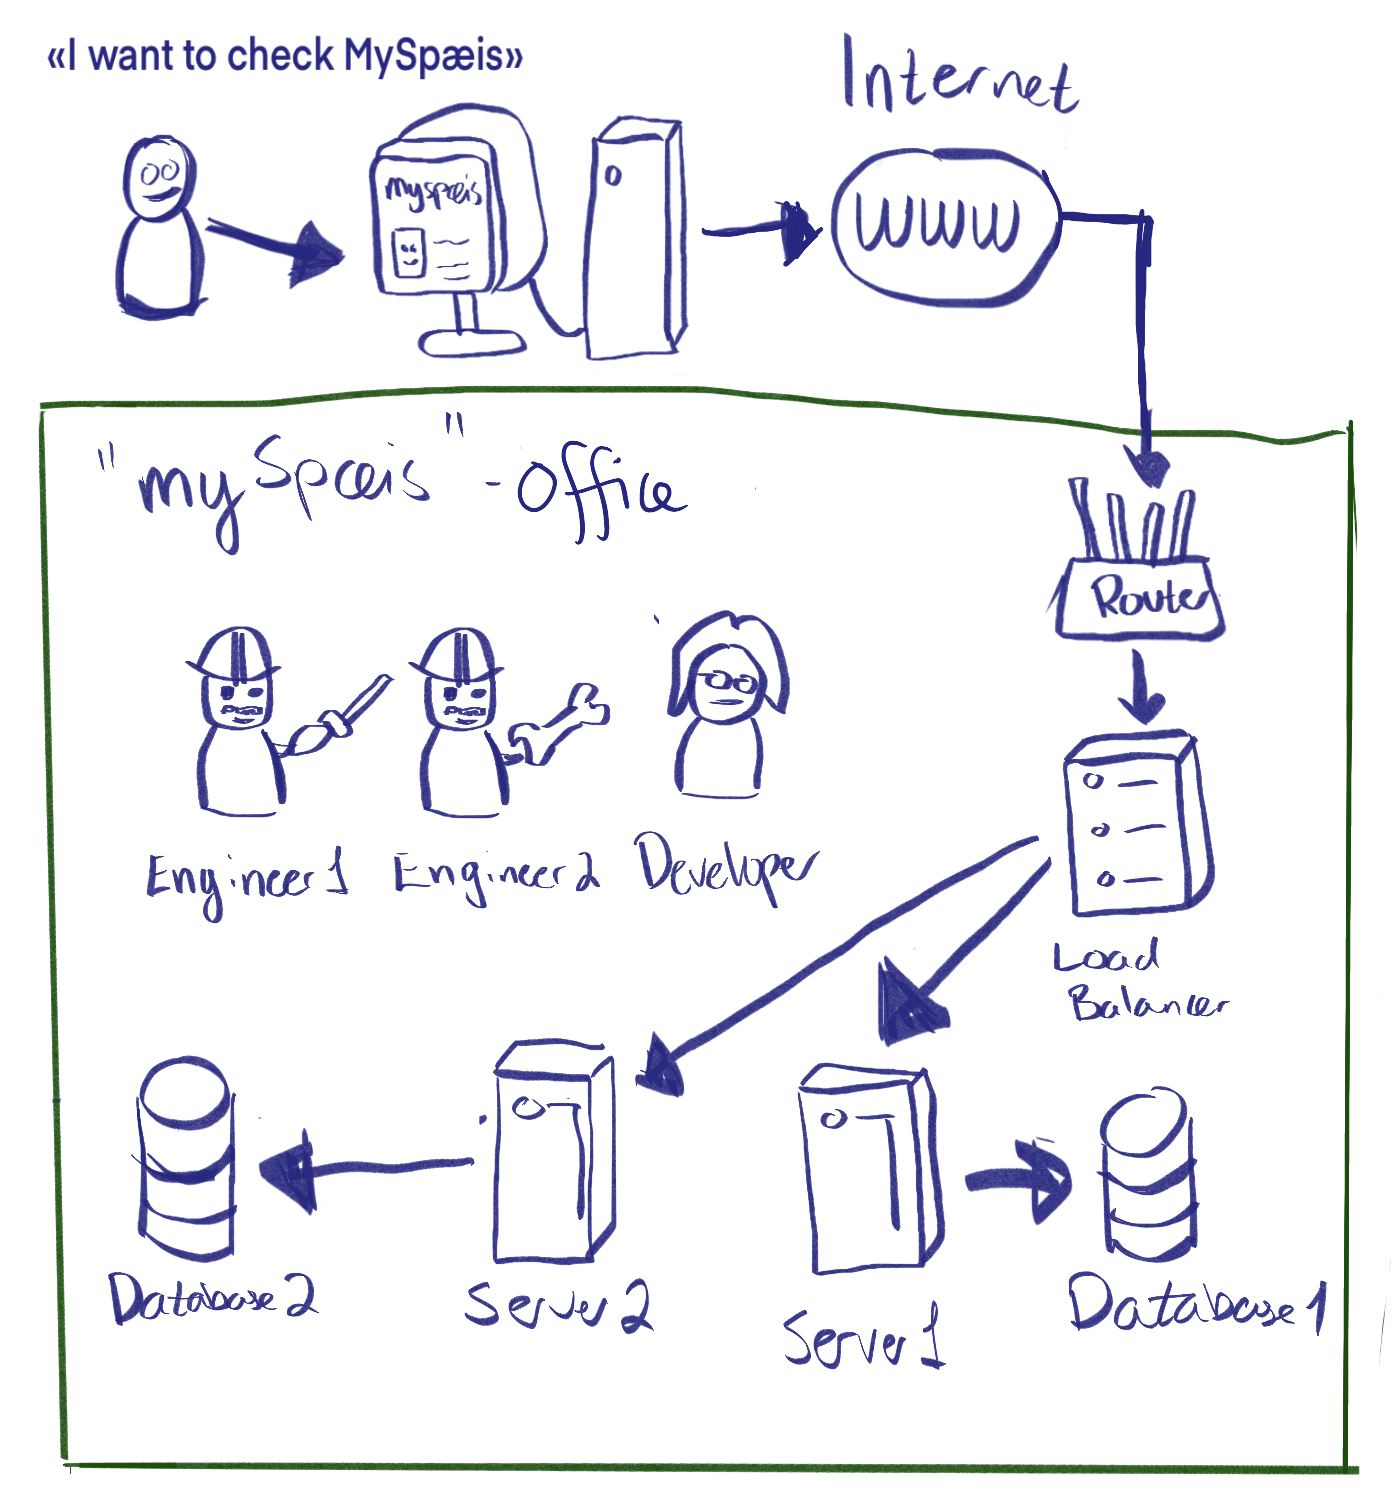
\includegraphics[width=0.7\columnwidth]{assets/2.1-before-the-waves-2.png}
  \caption{Example of a company that host their own infrastructure.}
  \label{fig:myspeis}
\end{figure}

Setting up such an infrastructure requires a significant cost, both
upfront for purchasing such a setup and for employing engineers who can
set up and maintain this. This puts a considerable financial strain on
organizations, and kept smaller companies without the financial backing
to invest in this at a disadvantage \citep{etroEconomicImpactCloud2009}.
Having to maintain infrastructure also poses a challenge when the
services start to gain traction. To meet the increased traffic on the
services, a company will have to scale up and extend the infrastructure,
which also can be expensive and difficult
\citep{armbrustViewCloudComputing2010}.

As a response to these challenges, some companies found a market for
taking on the responsibility of managing infrastructure, and offer
\ac{IaaS} to an evolving market that relies more and more on digital
solutions. \ac{IaaS} provides consumers with the ability to provision
computing resources where they can deploy and run software, including
operating systems and applications \citep{nist-def}. On these managed
infrastructures companies could deploy their services on top of virtual
machines that allowed more flexibility, and lowered the bar to new
companies.

\section{The First Wave: Virtual machines}
\label{sect:first-wave}

The start of cloud computing can be traced back to the emergence of
virtualization, more specifically virtual machines, a response to the
costly and complex nature of managing traditional, on-premise data
centers. During the mid-2000s, Amazon launched its subsidiary, Amazon
Web Services (AWS), who in turn launched Amazon S3 in March 2006,
followed by Elastic Compute Cloud (EC2) in August the same year
\citep{barrAmazonEC2Beta2006}. With these services, AWS positioned
itself as a pioneer in this space, marking a major turning point in
application development and deployment, and popularized cloud computing.
EC2, as an \ac{IaaS} platform, empowered developers to run virtual
machines remotely. (See \Cref{fig:feisbook} for an example of this kind
of architecture)

\begin{figure}[H]
\centering
  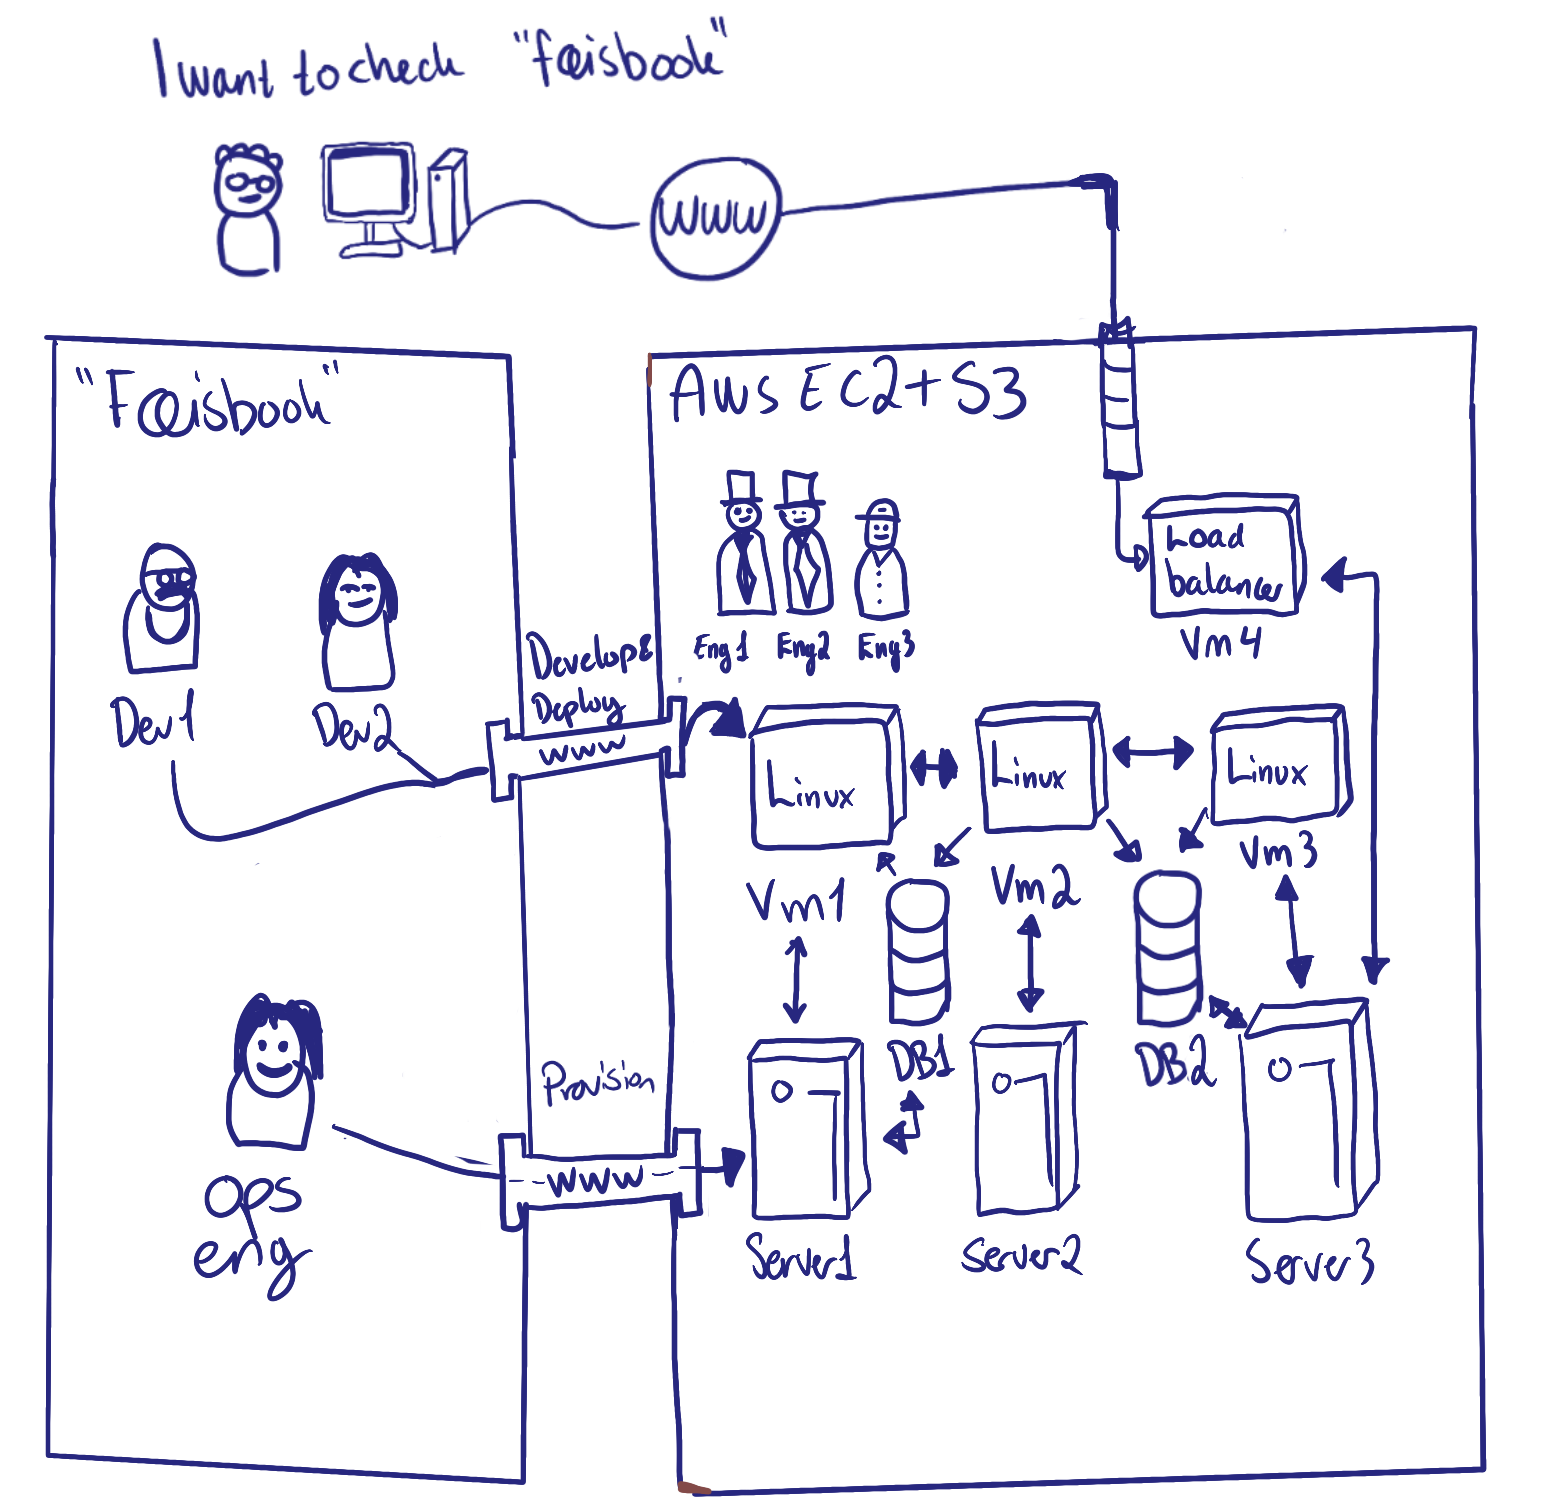
\includegraphics[width=0.7\columnwidth]{assets/2.2-first-wave-2.png}
  \caption{Example of ``Fæisbook`` building their services on EC2 and using S3
for storage.}
  \label{fig:feisbook}
\end{figure}

While similar services existed before 2006, with Amazon's existing large
customer base helped them gain significant traction, and ushered in a
the first era, or wave, of \emph{cloud computing}.

\section{The Second Wave: Containers}
\label{sect:second-wave}

As we entered the 2010s, the focus shifted from virtual machines to
containers, largely due to the limitations of VMs in efficiency,
resource utilization, and application deployment speed. Containers,
being a lightweight alternative to VMs, designed to overcome these
hurdles \citep{bao2016}.

In contrast to VMs, which require installation of resource-intensive
operating systems and minutes to start up, containers along with their
required OS components, could start up in seconds. Typically managed by
orchestration tools like Kubernetes\footnote{\url{https://kubernetes.io}},
containers enabled applications to package alongside their required OS
components, facilitating scalability in response to varying service
loads. Consequently, an increasing number of companies have since
established platform teams to build orchestrated developers platforms,
thereby simplifying application development in Kubernetes clusters. (See
\Cref{fig:docker} for an example where a fictive company
\texttt{WacDonalds} and their container workflow)

\begin{figure}[H]
\centering
  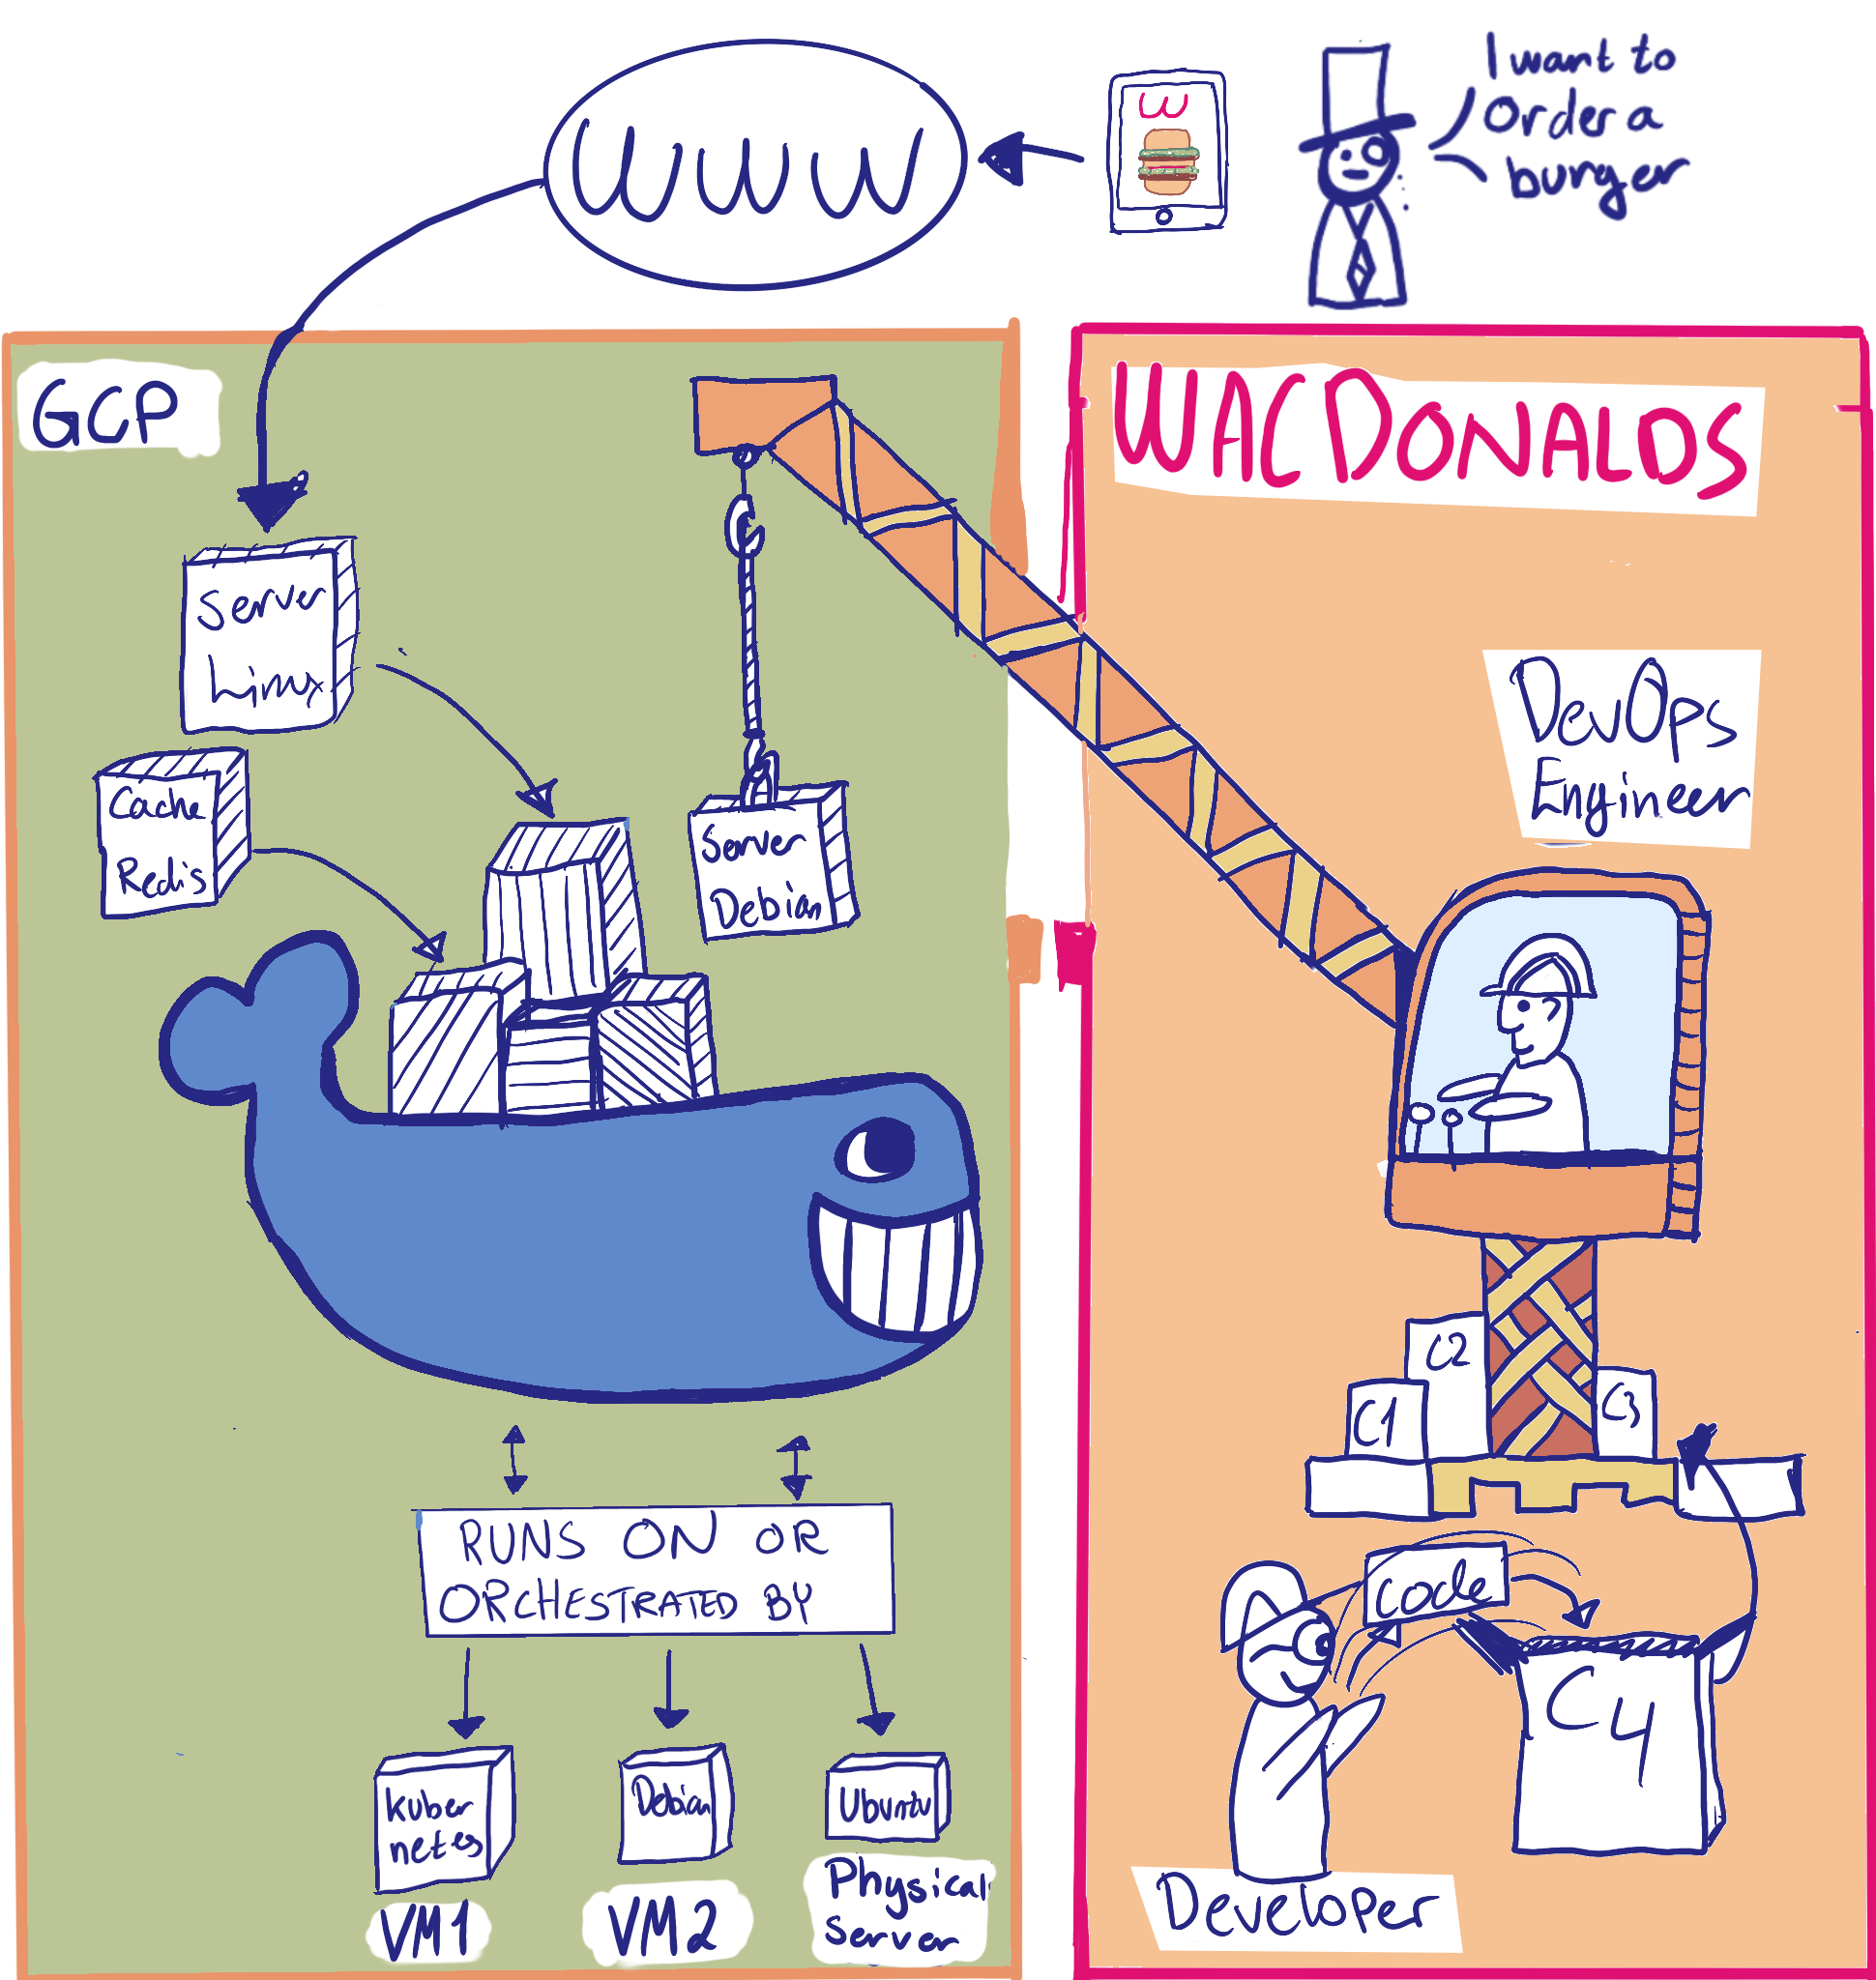
\includegraphics[width=0.8\columnwidth]{assets/2.3-second-wave-2.png}
  \caption{DevOps engineer deploying services as containers on \ac{GCP}.}
  \label{fig:docker}
\end{figure}

Containers are not a perfect solution however, and while they simplify
the means of developing and deploying applications, docker images can
easily reach Gigabytes in image size \citep{durieux2023}, can take a
long time to start up, and building applications that target multiple
platforms can be difficult.

These solutions are more efficient than manually installing an operating
system on a machine, but they still have leave a large footprint. Is
there a more efficient way to package and deploy our programs? \ac{Wasm}
and \ac{WASI}, as mentioned in epigraph of \cref{chap:intro}, has
positioned itself as a potential contender for how applications are
built, packaged and deployed to the cloud.

\section{The Third Wave: WebAssembly modules}
\label{sect:third-wave}

WebAssembly has had a surge of popularity the past three to four years
when developers discovered that what it was designed for - to truly run
safely inside the browser - translated well into a cloud native
environment as well. Containers have, with the benefits mentioned in
\cref{sect:second-wave}, had a positive impact on the cloud native
landscape. However, with the limitations - like large image sizes, slow
startups and complexity of cross-platform - there is space for exploring
alternative technologies for building our cloud-native applications.

WebAssembly is a compilation target with many languages adopting
support, and by itself, it is sandboxed to run in a WebAssembly \ac{VM}
without access to the outside world, meaning that it cannot access the
underlying system. This means that a ``vanilla'' WebAssembly module
cannot write to the file system, update a Redis cache or transmit a POST
request to another service.

To make this possible, the WebAssembly System Interface project was
created. This project allows developers to write code that compiles to
WebAssembly that can access the underlying system. This is the key
project that turned many developers onto the path of exploring
WebAssembly as a potential contender for building cloud applications.
With WebAssembly, developers can write programs in a programming
language that supports it as a compilation target, and build tiny
modules that can run on a WebAssembly runtime. These WebAssembly
runtimes can run on pretty much any architecture with ease, the
resulting binary size are quite small, and the performance is
near-native. These perks combined with the potential for reduced
overhead, smaller image sizes, and faster startup times make WebAssembly
and \ac{WASI} a promising candidate for the third wave of cloud compute
with a lower impact on the environment.

In summary, the three waves of cloud computing - virtual machines,
containers, and now \ac{Wasm} with \ac{WASI} - represent the industry's
pursuit of more efficient, scalable and reliable solutions for building
cloud applications. While each wave has attempted to tackle pressing
challenges of its time, it is exciting to see how \ac{Wasm} and
\ac{WASI} can be leveraged in this third wave and see if it is promise
of more efficient applications can lead to reducing the environmental
impact of ICT.

\newpage

\chapter{Background}
\label{chap:background}

\epigraph{\itshape 
Data has gravity, and that gravity pulls hard
}{David Flanagan}

\section{Cloud Computing Overview}
\label{sect:cloud-overview}

Cloud computing, commonly referred to as ``\emph{the cloud}'', refers to
the delivery of computing resources served over the internet, as opposed
to traditional on-premise hardware setups. The \ac{NIST} defines cloud
computing like so:

\begin{tcolorbox}[
  definitionstyle,
  title=NIST definition of Cloud Computing,
]
Cloud computing is a model for enabling ubiquitous, convenient, on-demand
network access to a shared pool of configurable computing resources (e.g.,
networks, servers, storage, applications, and services) that can be rapidly
provisioned and released with minimal management effort or service provider
interaction. \\

\hfill \citep{nist-def}

\end{tcolorbox}

Cloud computing traces its root back to the 1960s, with the Compatible
Time-Sharing System (CTSS) project at MIT, which demonstrated the
potential for multiple users accessing and sharing computing resources
simultaneously \citep{crisman1963}. While CTSS was a localized system,
it paved the way for the concept of shared computing resources, a
fundamental principle of cloud computing.

Over the following decades, advancements in networking, virtualization
and the ubiquity of the internet led to the development of today's
sophisticated cloud services. The term ``cloud computing'' was first
coined in the year 1996 by Compaq,
\citep{favaloroInternetSolutionsDivision1996}, but it was not until
Amazon launched its subsidiary \ac{AWS} in the 2006 that the adoption
became wide spread.

The launch of AWS's Amazon S3 cloud service in March 2006, followed by
Elastic Compute Cloud (EC2) in August the same year
\citep{barrAmazonEC2Beta2006}, marked a major turning point in
application development and deployment, and popularized cloud computing.
EC2, as an Infrastructure-as-a-Service platform, empowered developers to
run virtual machines remotely. By providing these services over the
internet on a pay-as-you-go basis, AWS drastically lowered the bar for
accessing computing resources, making it easier and more cost-effective
for businesses and developers to build and deploy applications without
the need for considerable upfront investment in hardware and
infrastructure.

With the success of AWS, other major technology companies saw their fit
to enter the cloud computing market. In 2008, Google launched the Google
App Engine \citep{mcdonaldIntroducingGoogleApp2008}, a platform for
building and hosting web applications in Google's data centers.
Microsoft followed with the launch of Azure in 2010, its cloud computing
platform that offers a range of services comparable to AWS.

The rapid growth of cloud computing also fueled the rise of DevOps
practices and containerization technologies like Docker, which
facilitate the development, deployment and management of applications on
the cloud. Orchestration tools like Docker Swarm and Kubernetes further
simplify the process of managing and scaling containerized applications
across cloud enviroments \citep{bernsteinContainersCloudLXC2014}.

Today, cloud computing has become an essential part of modern IT
infrastructure, where major cloud provides, like AWS, Microsoft and
Google, continue to innovate and expand their offerings. Cloud computing
has also enable new paradigms like serverless computing and edge
computing, allowing for even more efficient and distributed computing
models. \citep{baldiniServerlessComputingCurrent2017}

\section{Energy consumption and Sustainability in Cloud Computing}

A major drawback of cloud computing is the increasing energy consumption
required to power data centers. With the increased demand for energy
consumption, comes an increased impact on the environment. As mentioned
in \cref{chap:intro}, the ICT industry accounts for an estimated 2.1\%
to 3.9\% of global greenhouse emissions \citep{freitag2021}. According
to the International Energy Agency (IEA), data centers across the globe
consumed between from 240 to 340 TWh, accounting for 1 to 1.3\% of the
global electricity use.

In Norway, for example, Google is constructing a data center in Skien,
expected to be fully operational by 2026. As of April 2024, they have
been granted a capacity of 240 Megawatts, but they have applied for a
total capacity of 860 Megawatts
\citep{rivrudInvesteringenAvGooglesenter2024}. At full capacity at 860
MW, Google's data center is aiming to consume 7.5 TWh each year, and
according to Google's most recent sustainability report, they consumed a
total of 22.29 TWh globally in 2022 \citep{Google2023Environmental2023}.
In other words, in 2026 the data center in Skien alone is projected to
consume \textasciitilde33\% of the energy Google consumed globally in
2022. The energy consumption in Norway is projected to reach 150-158 TWh
in 2026 \citep{gunnerodStatnettAnalyse2022}, meaning that the data
center in Skien could account for 5\% of the energy consumption in the
country. \Cref{fig:skienvsnorway} below illustrates the amount of energy
the new data center will consume compared to Norway.

\vspace{0.25cm}

\begin{figure}

{\centering 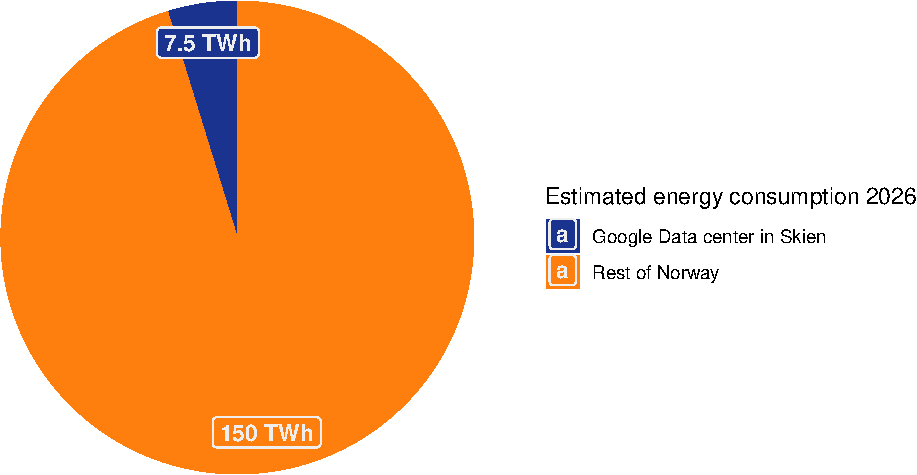
\includegraphics[width=0.8\linewidth]{thesis_files/figure-latex/skienvsnorway-1} 

}

\caption{Projected energy consumption in 2026: Skien data center and Norway.}\label{fig:skienvsnorway}
\end{figure}

\todo[inline=true]{Consider this feedback from Michael: Google also does not
make it rain more. If Google come and buys all the green energy in the area, it
will just mean that others will use more black energy. They don't build new
infrastructure. And this is only for Googles "usage". Not the users and network
infrastructure.}

The flipside of this, is that Google is commited to reach a net-zero
carbon footprint by 2030, and the data center in Skien is built to
reflect this. Google has been carbon neutral since 2007 and has matched
100\% of its annual electricity consumption with renewable energy since
2017 \citep{googleTrackingOurCarbonFree}. Norway's abundant hydropower,
rising wind power production, investment into solar energy and other
renewable energy sources make it an ideal location for building data
centers aiming to be powered by renewable energy
\citep{norwegian-energyElectricityProduction2023}.

Like Google, other major cloud providers have set ambitious targets for
renewable energy adoption and have invested in large-scale renewable
projects. Microsoft has committed to shifting to 100\% renewable energy
by 2025 for all its data centers, buildings and campuses, and to be
carbon \emph{negative} by 2030 \citep{smithMicrosoftWillBe2020}, while
Amazon has pledged to transition to 100\% renewable energy by 2030 for
its cloud subsidiary and to have a net-zero carbon footprint by 2040
\citep{amazonClimatePledge2019}. These efforts have contributed to
reducing greenhouse gas emissions in the cloud computing industry, but
this commitment is not universally adopted, and many data centers still
rely on electricity generated by fossil fuels, a leading contributor to
climate change \citep{mytton2020}.

Several factors make up the energy consumption required to service a
data center. One of these factors is cooling down the servers while
running, and a study from 2017 discovered that cooling accounted for
about 38\% of total energy consumption in data centers, ranging from
21\% to 61\% depending the effectiveness of the facility's heating,
ventilation, and air conditioning (HVAC) system
\citep{niReviewAirConditioning2017}.

One innovative example of attempting to mitigate the environmental
impact of cooling data centers can be found by data center providers
like DeepGreen\footnote{\url{https://deepgreen.energy/faqs/}}, who
submerge their servers into dielectric fluid, which gets warmed up by
the excess heat of the computers. This heat is then transferred to a
host's hot water system via a heat exchange and used for heating up
swimming pools in London. Another broad strategy cloud providers opt for
is the implementation of power management techniques, such as dynamic
voltage and frequency scaling (DVFS), which adjusts the power
consumption of servers based on workload demands
\citep{beloglazovEnergyawareResourceAllocation2012}.

Virtualization and resource pooling, two key components of cloud
computing, also contribute to energy efficiency. By consolidating
virtual machines onto shared physical servers, cloud providers are able
to improve resource utilization and reduce the energy consumption of
their data centers. \citep{beloglazovEnergyawareResourceAllocation2012}

\section{Virtualization and Virtual Machines}
\label{sect:virtual}

Virtualization is the process of creating a virtual version of a
physical resource, such as an operating system, a server, a storage
device, or a network resource
\citep{chiuehSurveyVirtualizationTechnologies2005}. Virtualization allow
multiple virtual instances to share the underlying physical hardware,
enabling more efficient resource utilization and consolidation.

One of the most common forms of virtualization is the creation of
\ac{VMs}. \citet{barhamXenArtVirtualization2003} described that a
virtual machine is a software-based emulation of a physical computer
system, including its processor, memory, storage, and network
interfaces. Furthermore they describe that \ac{VMs} run on top of a
hypervisor, a software layer that manages and allocates the physical
hardware resources to the virtual machines.

\Cref{vm-figure} below illustrates virtual machines running in such an
environment.

\begin{figure}[H]
\centering
  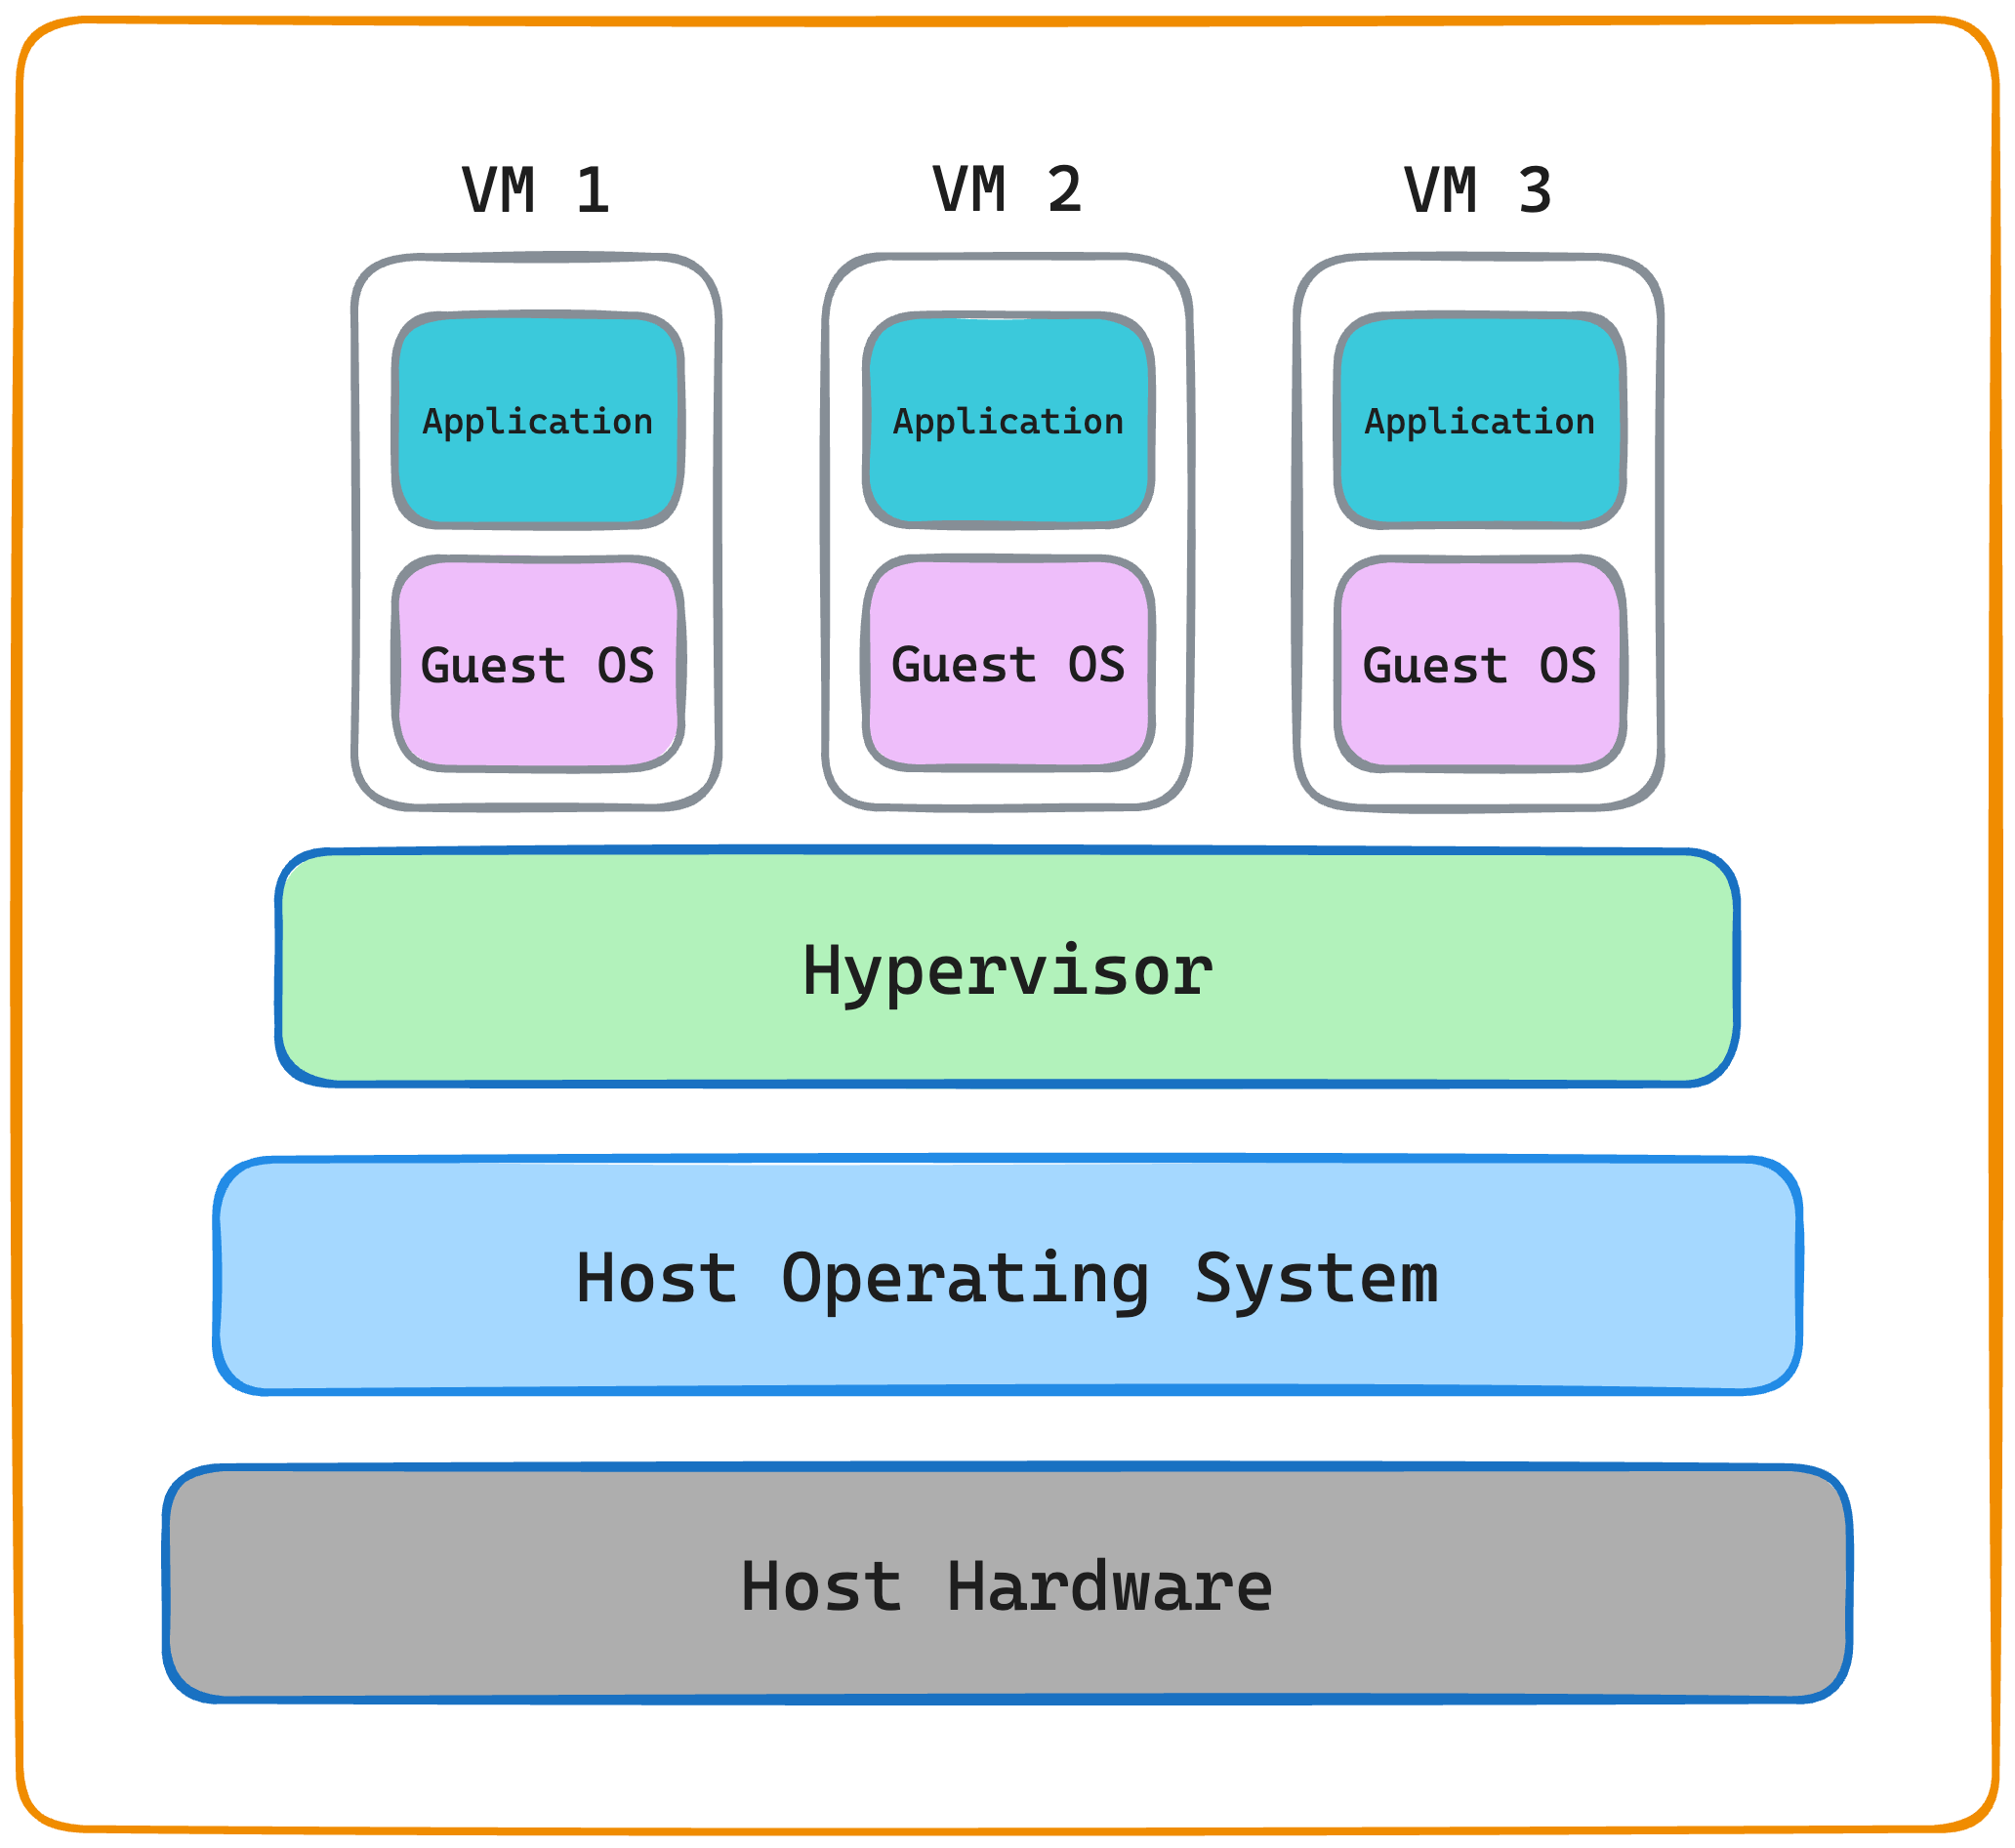
\includegraphics[width=0.7\columnwidth]{assets/3.2-vm-figure.png}
  \caption{Virtual machines running on top of Hypervisor on a computer.}
  \label{vm-figure}
\end{figure}

By consolidating multiple servers through virtualization and running
them on the same physical server, data centers can drastically decrease
the number of physical machines required, leading to a reduction in
energy consumption \citep{kaplanRevolutionizingDataCenter2008}.

\section{Containers and Container orchestration}
\label{sect:containers}

While virtual machines provide isolation at the hardware level,
containers offer a more lightweight form of virtualization by isolating
applications at the operating system level
\citep{merkelDockerLightweightLinux2014}. Containers share the host
operating system's kernel, enabling them to be more lightweight and
efficient compared to traditional virtual machines. They can run
physical servers, as well as on \ac{VMs}
\citep{bernsteinContainersCloudLXC2014}.

\citet{merkelDockerLightweightLinux2014} also explains that containers
package an application and its dependencies into a single unit. This
includes libraries, configuration files and other necessary files. This
allows applications to be deployed consistently across different
environments, ensuring predictable behavior and reducing compatibility
issues \citep{sergeevDockerContainerPerformance2022}

By enabling more granular and efficient use of system resources,
containers contribute to lower energy usage compared to virtual machines
due to their lightweight nature and faster startup times
\citep{shirinbabPerformanceEvaluationContainers2020}. The adoption of
containerization technologies have been shown to optimize energy costs,
as containers allow for a higher density of applications running on the
same physical hardware without the overhead associated with full
virtualization
\citep{cuadrado-corderoComparativeExperimentalAnalysis2018}.

Docker is one of the most widely adopted container platforms, providing
tools for building, shipping, and running applications in containers
\citep{merkelDockerLightweightLinux2014}. Docker containers are based on
open standards and can run on various operating systems and cloud
platforms \citep{sergeevDockerContainerPerformance2022}.
\Cref{container-figure} below illustrates how containers run ontop of a
Docker Engine on a virtual or physical machine.

\begin{figure}[H]
\centering
  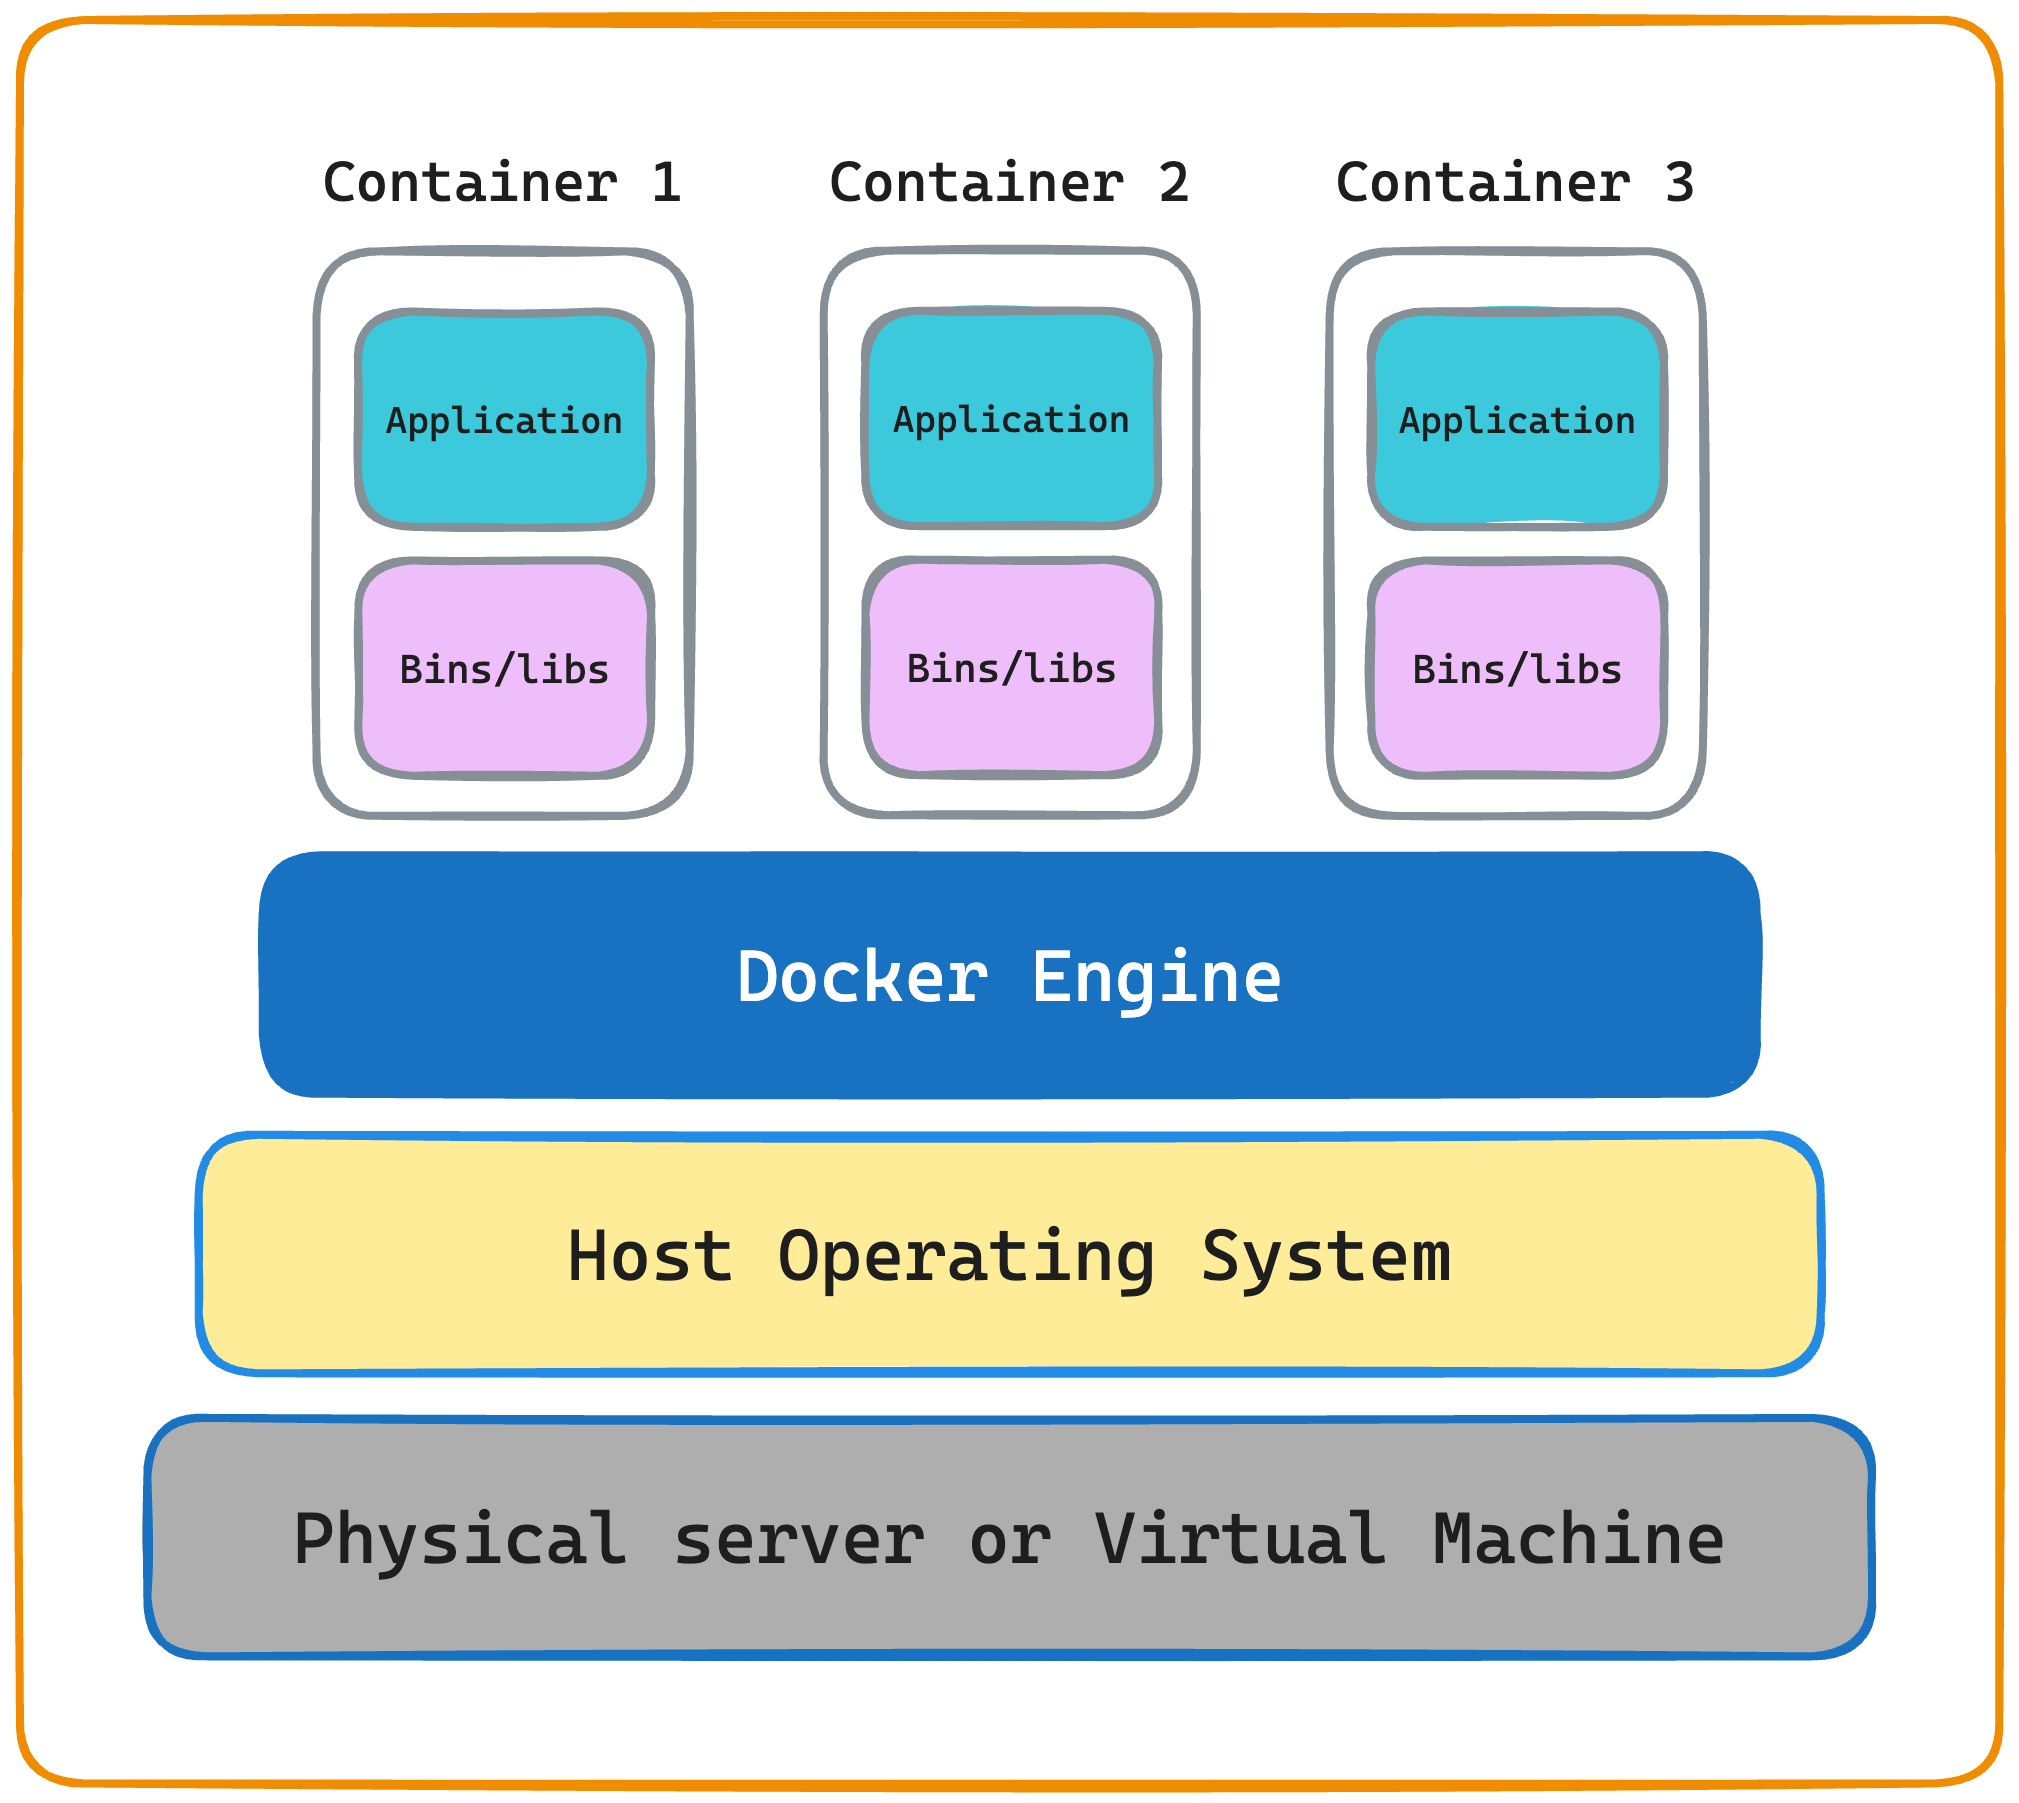
\includegraphics[width=0.7\columnwidth]{assets/3.3-container-figure.png}
  \caption{Containers running on the Docker Engine}
  \label{container-figure}
\end{figure}

As the number of containers in an environment grows, managing and
orchestrating them becomes increasingly complex. Container orchestration
tools, such as Kubernetes and Docker Swarm, help automate the
deployment, scaling, and management of containerized applications across
multiple hosts \citep{burnsBorgOmegaKubernetes2016}.

These tools provide features like:

\begin{enumerate}
\def\labelenumi{\arabic{enumi}.}
\tightlist
\item
  Automated deployment and scaling: Containers can be automatically
  provisioned, scaled up or down based on demand, and load-balanced
  across multiple hosts \citep{burnsBorgOmegaKubernetes2016}.
\item
  Self-healing and monitoring: Orchestration tools can monitor the
  health of containers and automatically restart or reschedule them in
  case of failures \citep{kubernetesKubernetes}.
\item
  Service discovery and load balancing: Applications running in
  containers can be easily discovered and accessed by other services,
  enabling microservice architectures \citep{kubernetesKubernetes}.
\end{enumerate}

Container orchestration has become an essential component of modern
cloud-native architectures, enabling efficient management and scaling of
containerized applications in dynamic environments.

\section{Serverless Computing}

Serverless computing has emerged as an alternative to traditional
infrastructure management approahces, such as managing physical servers
or building developer platforms as described in \Cref{sect:containers}
\citep{baldiniServerlessComputingCurrent2017}. In serverless computing,
the underlying infrastrucutre is abstracted away, allowing developers to
focus on writing code and deploying programs without the need to
provision or manage servers
\citep{baldiniServerlessComputingCurrent2017,robertsServerlessArchitectures2018}.
\citet{castroRiseServerlessComputing2019} defines serverless as such:

\begin{tcolorbox}[
  definitionstyle,
  title=Serverless definition,
]
Serverless computing is a platform that hides server usage from
developers and runs code on-demand automatically scale and billed only for the
code running. \\

\hfill \citep{castroRiseServerlessComputing2019}

\end{tcolorbox}

According to \citet{baldiniServerlessComputingCurrent2017}, in a
serverless model, the cloud provider is responsible for managing the
infrastructure, including resource allocation, scaling, and maintenance.
This approach enables more efficient resource utilization, as resources
are dynamically allocated based on demand. Furthermore, developers can
deploy containers or functions independently, promoting modularity and
scalability.

On top of this, severless computing offers several more benefits,
including:

\begin{enumerate}
\def\labelenumi{\arabic{enumi}.}
\tightlist
\item
  Reduced operational overhead: Developers do not need to manage servers
  or infrastructure, freeing up time and resources for application
  development \citep{baldiniServerlessComputingCurrent2017}.
\item
  Faster time-to-market: With serverless, developers can quickly deploy
  and iterate on functions without the need for time consuming
  infrastructure setup \citep{adzicServerlessComputingEconomic2017}.
\item
  Cost efficiency: Serverless platforms typically employ a pay-per-use
  pricing model, where users are charged based on the actual execution
  time and resources consumed by their applications
  \citep{eismannReviewServerlessUse2021}.
\end{enumerate}

However, serverless architectures also introduce certain challenges,
such as:

\begin{enumerate}
\def\labelenumi{\arabic{enumi}.}
\tightlist
\item
  Potential vendor lock-in: Serverless platforms may have
  provider-specific APIs and services, which can make it challenging to
  change providers or migrate applications
  \citep{gottliebServerlessDataLockin2018}.
\item
  Cold start latencies: Containers or functions that have not beeen
  invoked recently may experience longer startup times, cold starts,
  which can impact application performance
  \citep{golecColdStartLatency2023}.
\item
  Resource overhead and efficiency: Serverless platforms typically rely
  on containerization technologies, such as Docker, to encapsulate and
  isolate function executions. The use of containers can introduce
  resource overhead and impact the efficiency of serverless applications
  \citep{akkusSANDHighPerformanceServerless2018}.
\end{enumerate}

Examples of widely used platforms that build on the serverless model can
be found at the major cloud providers, like Google Cloud Run\footnote{\url{https://cloud.google.com/run}},
\ac{AWS} Fargate\footnote{\url{https://aws.amazon.com/fargate/}} and
Microsoft's \ac{ACI}\footnote{\url{https://azure.microsoft.com/en-us/products/container-instances}}.
These three example platforms allow developers to deploy containers onto
the cloud without worrying about orchestration behind the scenes.

\subsection{Functions-as-a-Service}

\ac{FaaS} is a cloud computing model, derived from serverless, that
allows developers to execute individual functions in response to events
or triggers without needing to manage the underlying infrastructure
\citep{sewakWinningEraServerless2018}.

Examples of these \ac{FaaS} platforms among the big three cloud
providers are; \ac{AWS} Lambda\footnote{\url{https://aws.amazon.com/lambda/}},
Google Cloud Functions\footnote{\url{https://cloud.google.com/functions}},
and Microsoft's Azure Functions\footnote{\url{https://azure.microsoft.com/en-us/products/functions}}.
On FaaS platforms like these, developers write and deploy small,
self-contained functions that perform specific tasks. These functions
are typically stateless and can be written in various programming
languages supported by the FaaS provider
\citep{baldiniServerlessComputingCurrent2017}.

When a function is triggered, the FaaS platform automatically allocates
the necessary resources to execute the function, such as CPU, memory,
and network bandwidth. The platform also handles the scaling of the
function based on the incoming requests, ensuring that the function can
handle varying workloads by itself
\citep{mcgrathServerlessComputingDesign2017}.

FaaS platforms often utilize container technology, like Docker, to
provide an isolated environment for each function execution. Containers
offer several benefits, such as fast startup times, efficient resource
utilization, and the ability to package functions with their
dependencies \citep{vaneykServerlessMorePaaS2018}. However, the use of
containers in FaaS also introduce some challenges including, cold start
latency and the overhead associated with container initialization and
management \citep{wangPeekingCurtainsServerless2018}.

Cold start latency refers to the time it takes for a FaaS platform to
provision a new container instance when a function is invoked after a
period of inactivity. This latency can be significant, especially for
applications with strict performance requirements
\citep{wangPeekingCurtainsServerless2018}. The limitations of containers
in FaaS environments have led to the exploration of alternative
approaches, such as using \ac{Wasm} and \{WASI\}. As Solomon Hykes, the
creator of Docker, stated:

\begin{displayquote}
\textit{ ``If WASM+WASI existed in 2008, we wouldn't have needed to create Docker.
That's how important it is. WebAssembly on the server is the future of cloud
computing. A standardized system interface was the missing link. Let's hope WASI
is up to the task.`` \citep{hykesOne2019} }
\end{displayquote}

This statement highlights the potential of \ac{Wasm} and \ac{WASI} to
face the challenges with containers in FaaS and to provide a more
efficient and platform-agnostic approach to serverless computing, a
potential explored and supported by
\citet{kjorveziroskiEvaluatingWebAssemblyOrchestrated2022}.

\section{WebAssembly and WASI}
\label{sect:wasmwasi}

WebAssembly, commonly referred to as Wasm, is a modern binary
instruction format that has risen to prominence as a versatile
technology across a diverse amount of computing environments,
originating in the web browser. This section introduces the project that
WebAssembly evolved from - \emph{asm.js} - and illustrate how
WebAssembly lets developers write programs in a high-level language and
run them across a multitude of platforms.

\subsection{asm.js}
\label{subsect:asm}

Mozilla released the first version of asm.js in 2013, and it was
designed be a subset of JavaScript, allowing web applications written in
other languages than JavaScript, such as C or C++, to run in the
browser. The intention of asm.js was to enable web applications to run
at performance closer to native code than applications written in
standard JavaScript A simplified flow for how source code written in
C/C++ is compiled to bytecode that can be executed in the browser can be
found in figure \ref{fig:asm-figure} below.

\begin{figure}[H]
\centering
  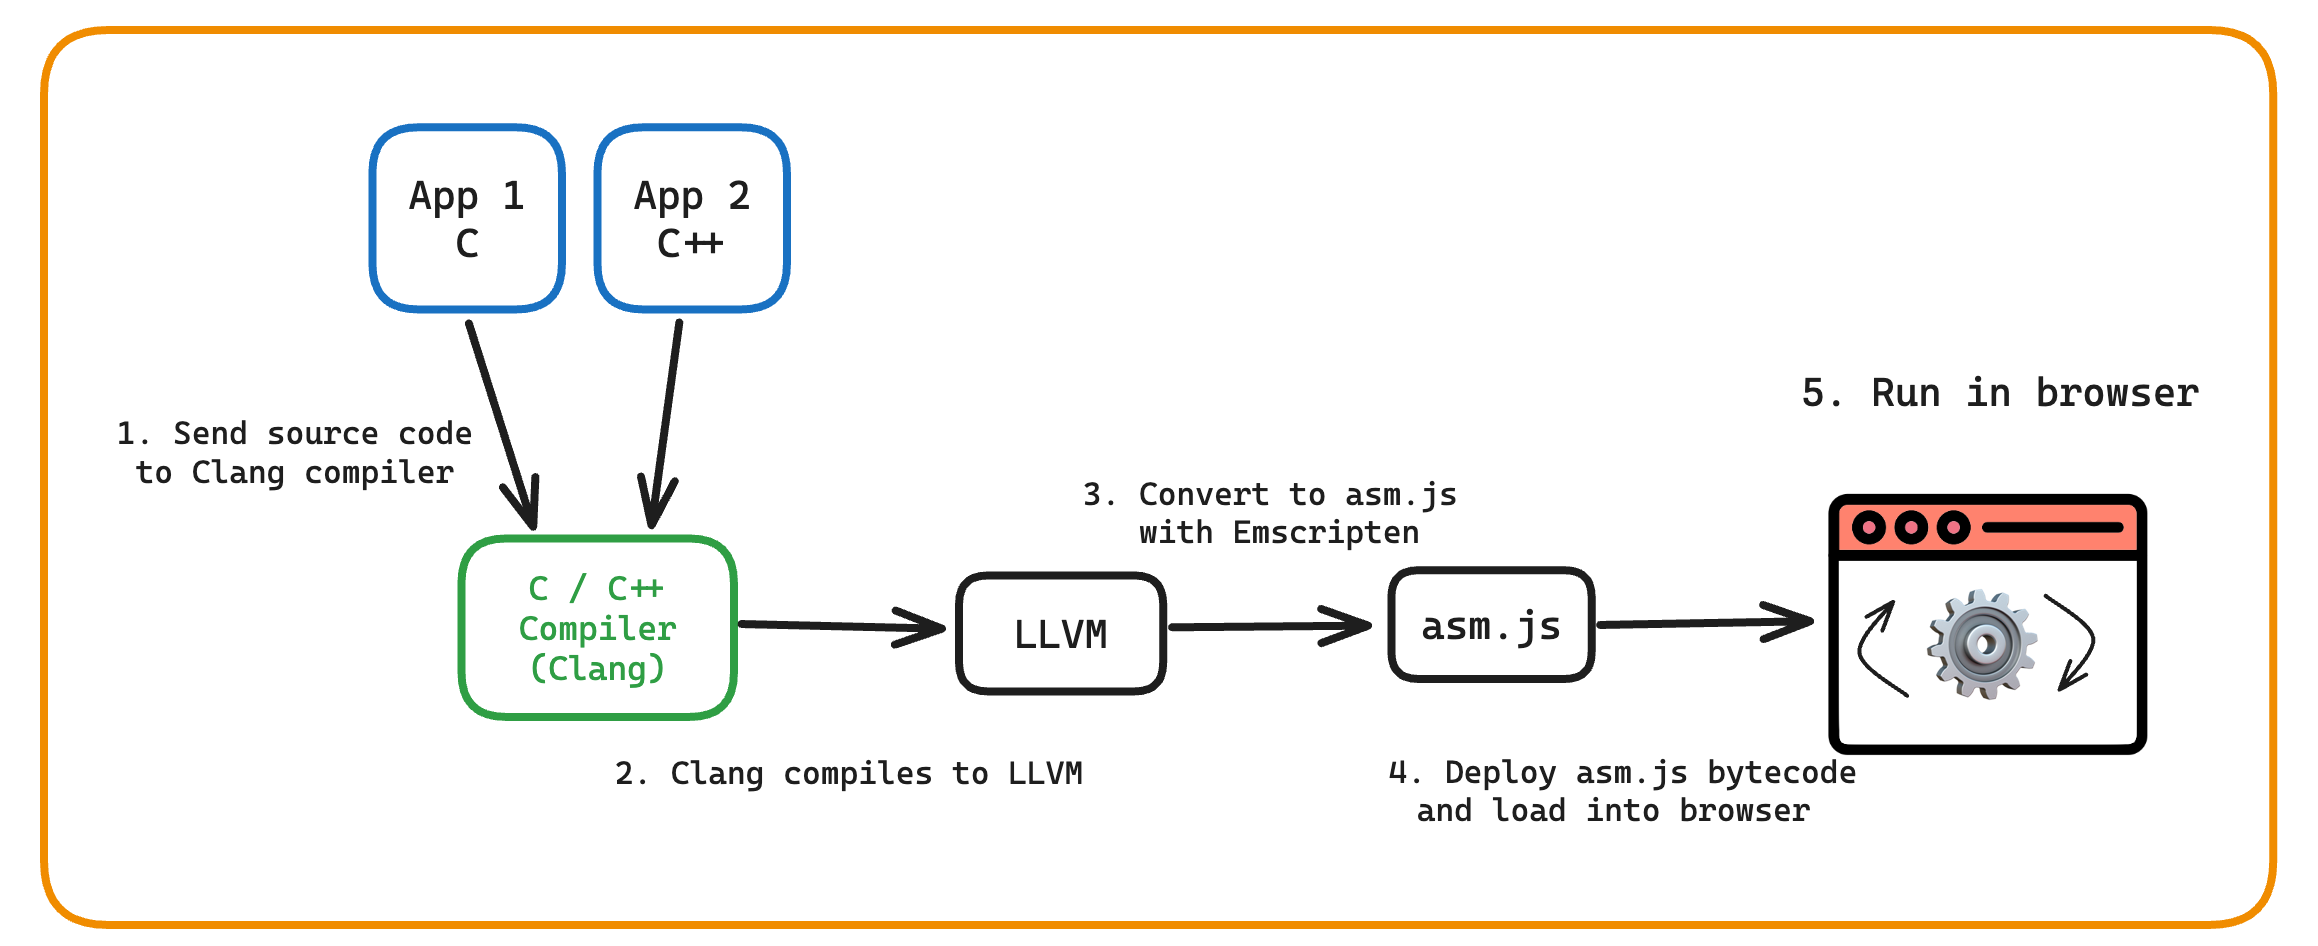
\includegraphics{assets/asm.js-figure.png}
\caption{Source code in C/C++ compiled to asm.js and run in browser}\label{fig:asm-figure}
\end{figure}

While asm.js was a great leap forward, being a subset of JavaScript
limited its scope, leading to its deprecation in 2017 and the
development of a more efficient and portable format
\citep{webassembly.orgFAQWebAssembly}.

\subsection{WebAssembly}

The team at Mozilla built upon the lessons learned from asm.js and went
on to develop WebAssembly, launching the first public version in 2017.
WebAssembly is a low-level code format designed to serve as a
compilation target for high-level programming languages
\citep{haasBringingWebSpeed2017}. It is a binary format that gets
executed by a stack-based virtual machine, comparable to how Java
bytecode runs on the \ac{JVM} \citep{haasBringingWebSpeed2017}. In
\Cref{fig:wasm-browser} below, a simplified flow for compiling web
applications written in different languages can be compiled and run
inside a web browser.

\begin{figure}[H]
\centering
  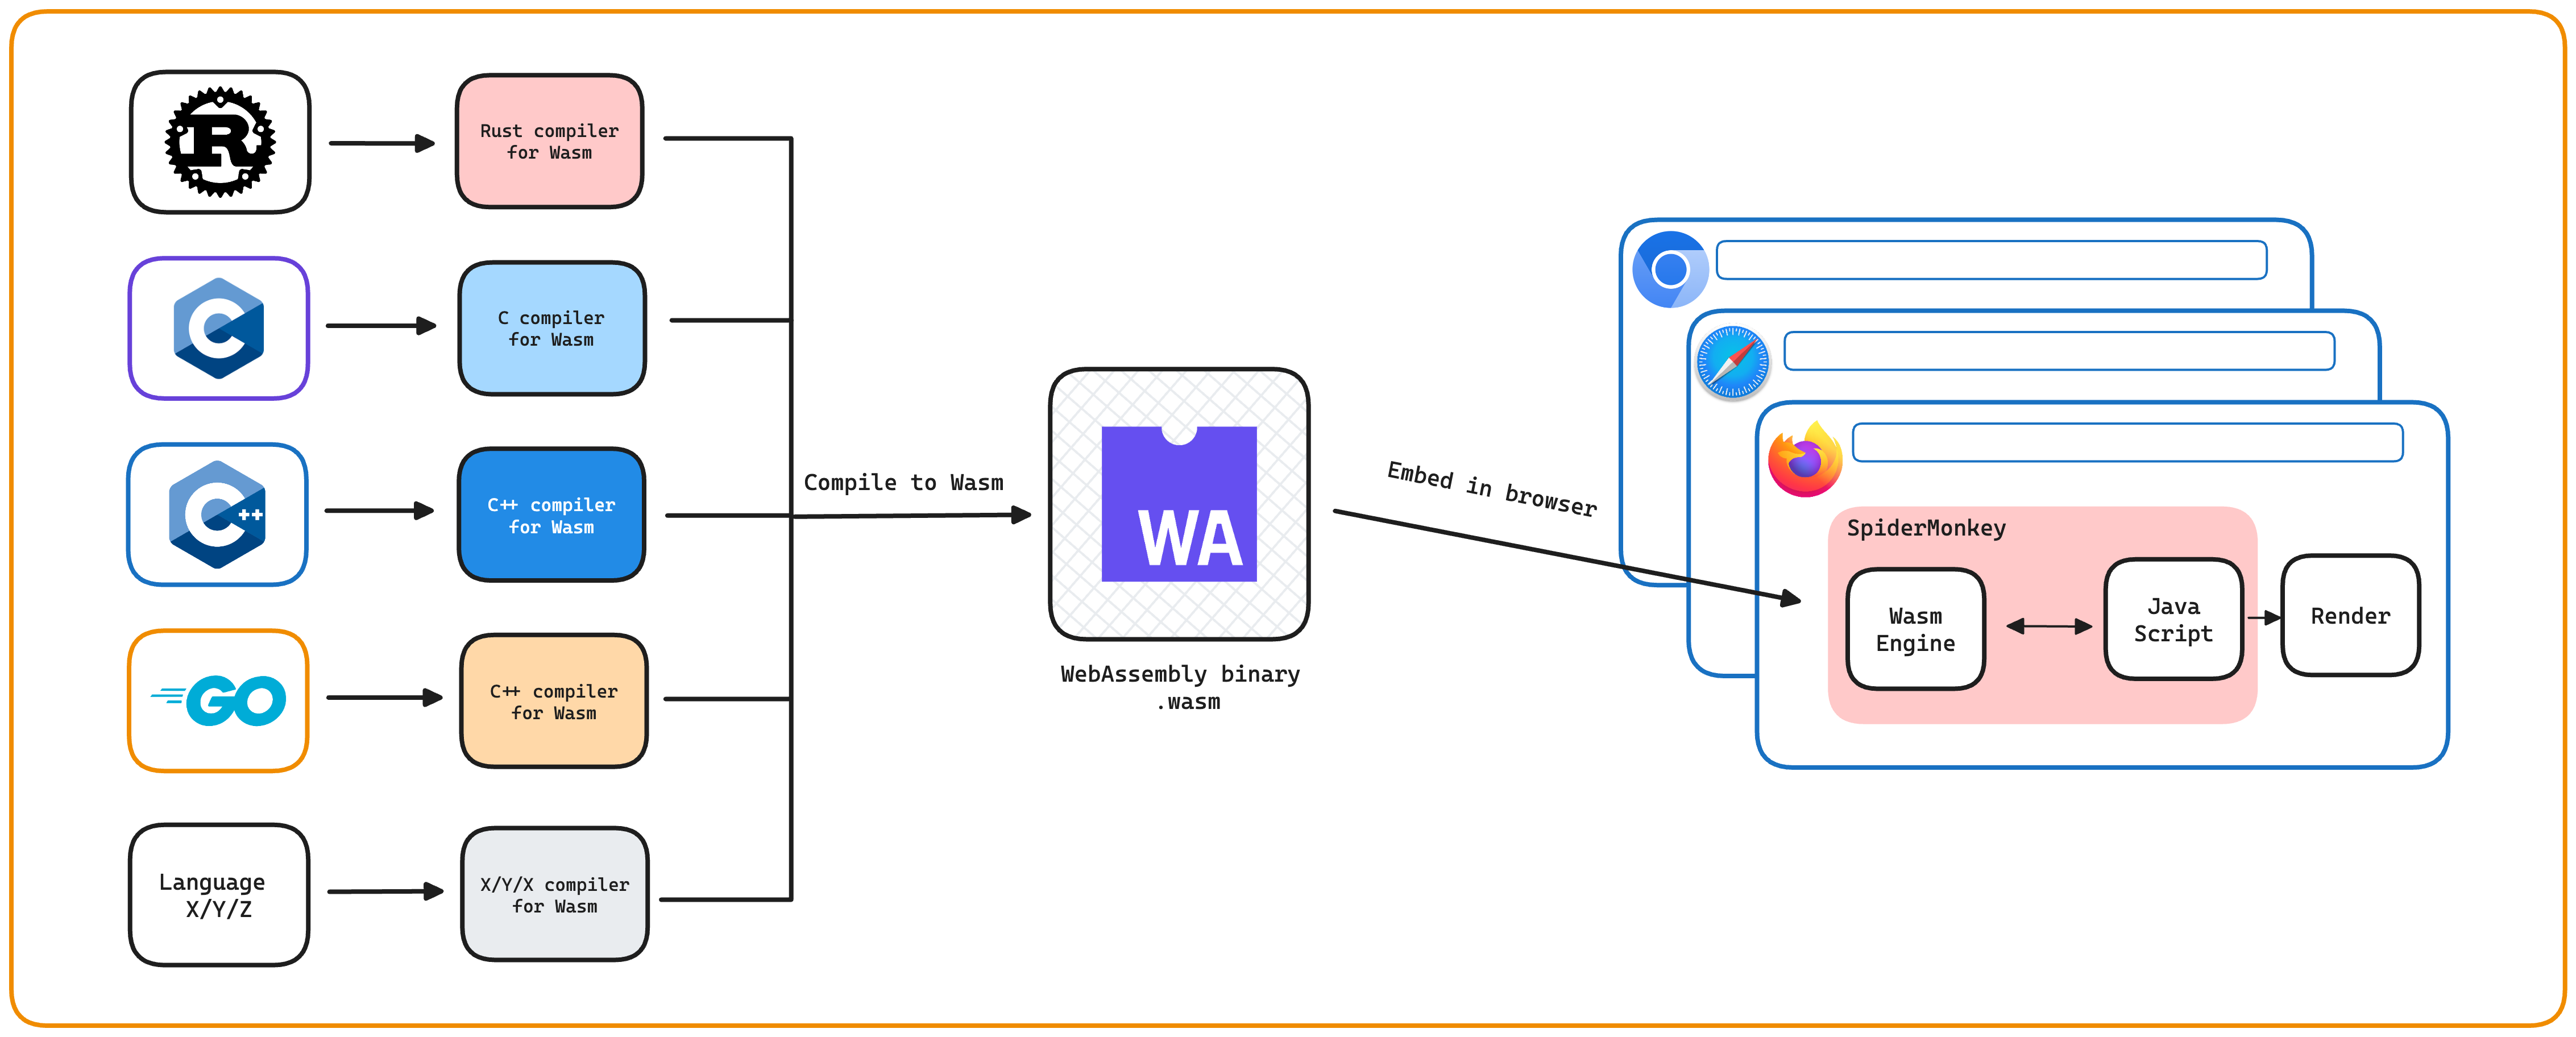
\includegraphics{assets/wasm-browser.png}
  \caption{Source code compiled to WebAssembly and embedded in browser}
  \label{fig:wasm-browser}
\end{figure}

According to \citet{haasBringingWebSpeed2017}, some key features of
\ac{Wasm} include:

\begin{enumerate}
\def\labelenumi{\arabic{enumi}.}
\tightlist
\item
  Portability: \ac{Wasm} is designed to be a portable binary instruction
  format that can run on various hardware platforms and operating
  systems. This portability is achieved through a hardware-independent
  instruction set and a sandboxed execution environment.
\item
  Performance: \ac{Wasm} aims to achieve performance close to native
  code by taking advantage of common hardware capabilities like a simple
  load-store architecture, single stating assignment form, and
  ahead-of-time compilation.
\item
  Security: \ac{Wasm} modules are executed in a sandboxed environment,
  which isolates them from the host system and enforces strict hardware
  limits on memory access and control flow. This helps mitigate security
  vulnerabilities associated with traditional web applications.
\item
  Open and Modular design: \ac{Wasm} is an open standard with a modular
  design, allowing for extensions and integration with various
  programming languages and tools. This modularity enables \ac{Wasm} to
  be used in a wide range of applications beyond just web browsers.
\item
  Efficient compression: The binary format of \ac{Wasm} is designed to
  be efficiently compressed, reducing the size of the distributed code
  and improving download times, especially in resource-constrained
  devices like mobile devices.
\end{enumerate}

By addressing performance, security and portability concerns, \ac{Wasm}
offers an alternative to traditional approaches for running untrusted
code on the web and in other computing environments, such as cloud and
edge computing \citep{haasBringingWebSpeed2017}.

\subsection{WebAssembly System Interface}

While \ac{Wasm} was initially designed to run in web browsers, its
potential for use in other environments, such as cloud and edge
compuitng, led to the development of the WebAssembly System Interface.
\ac{WASI} is a modular system interface that provides a standardized set
of functions for interacting with the host operating system, enabling
\ac{Wasm} modules to run outside of web browsers \citep{WASIDev}.

\ac{WASI} defines a set of APIs for performing tasks like file system
operations, networking, and other system-level operations, allowing
\ac{Wasm} modules to be portable across different platforms and
environments \citep{WASIDev}. It's first iteration aimed to be implement
as many POXIS-like features as possible, but has since extended beyond
this and in their latest Preview 2, they have implemented support for
websockets and HTTP interfaces \citep{WASIPreview2README}.

\begin{figure}[H]
\centering
  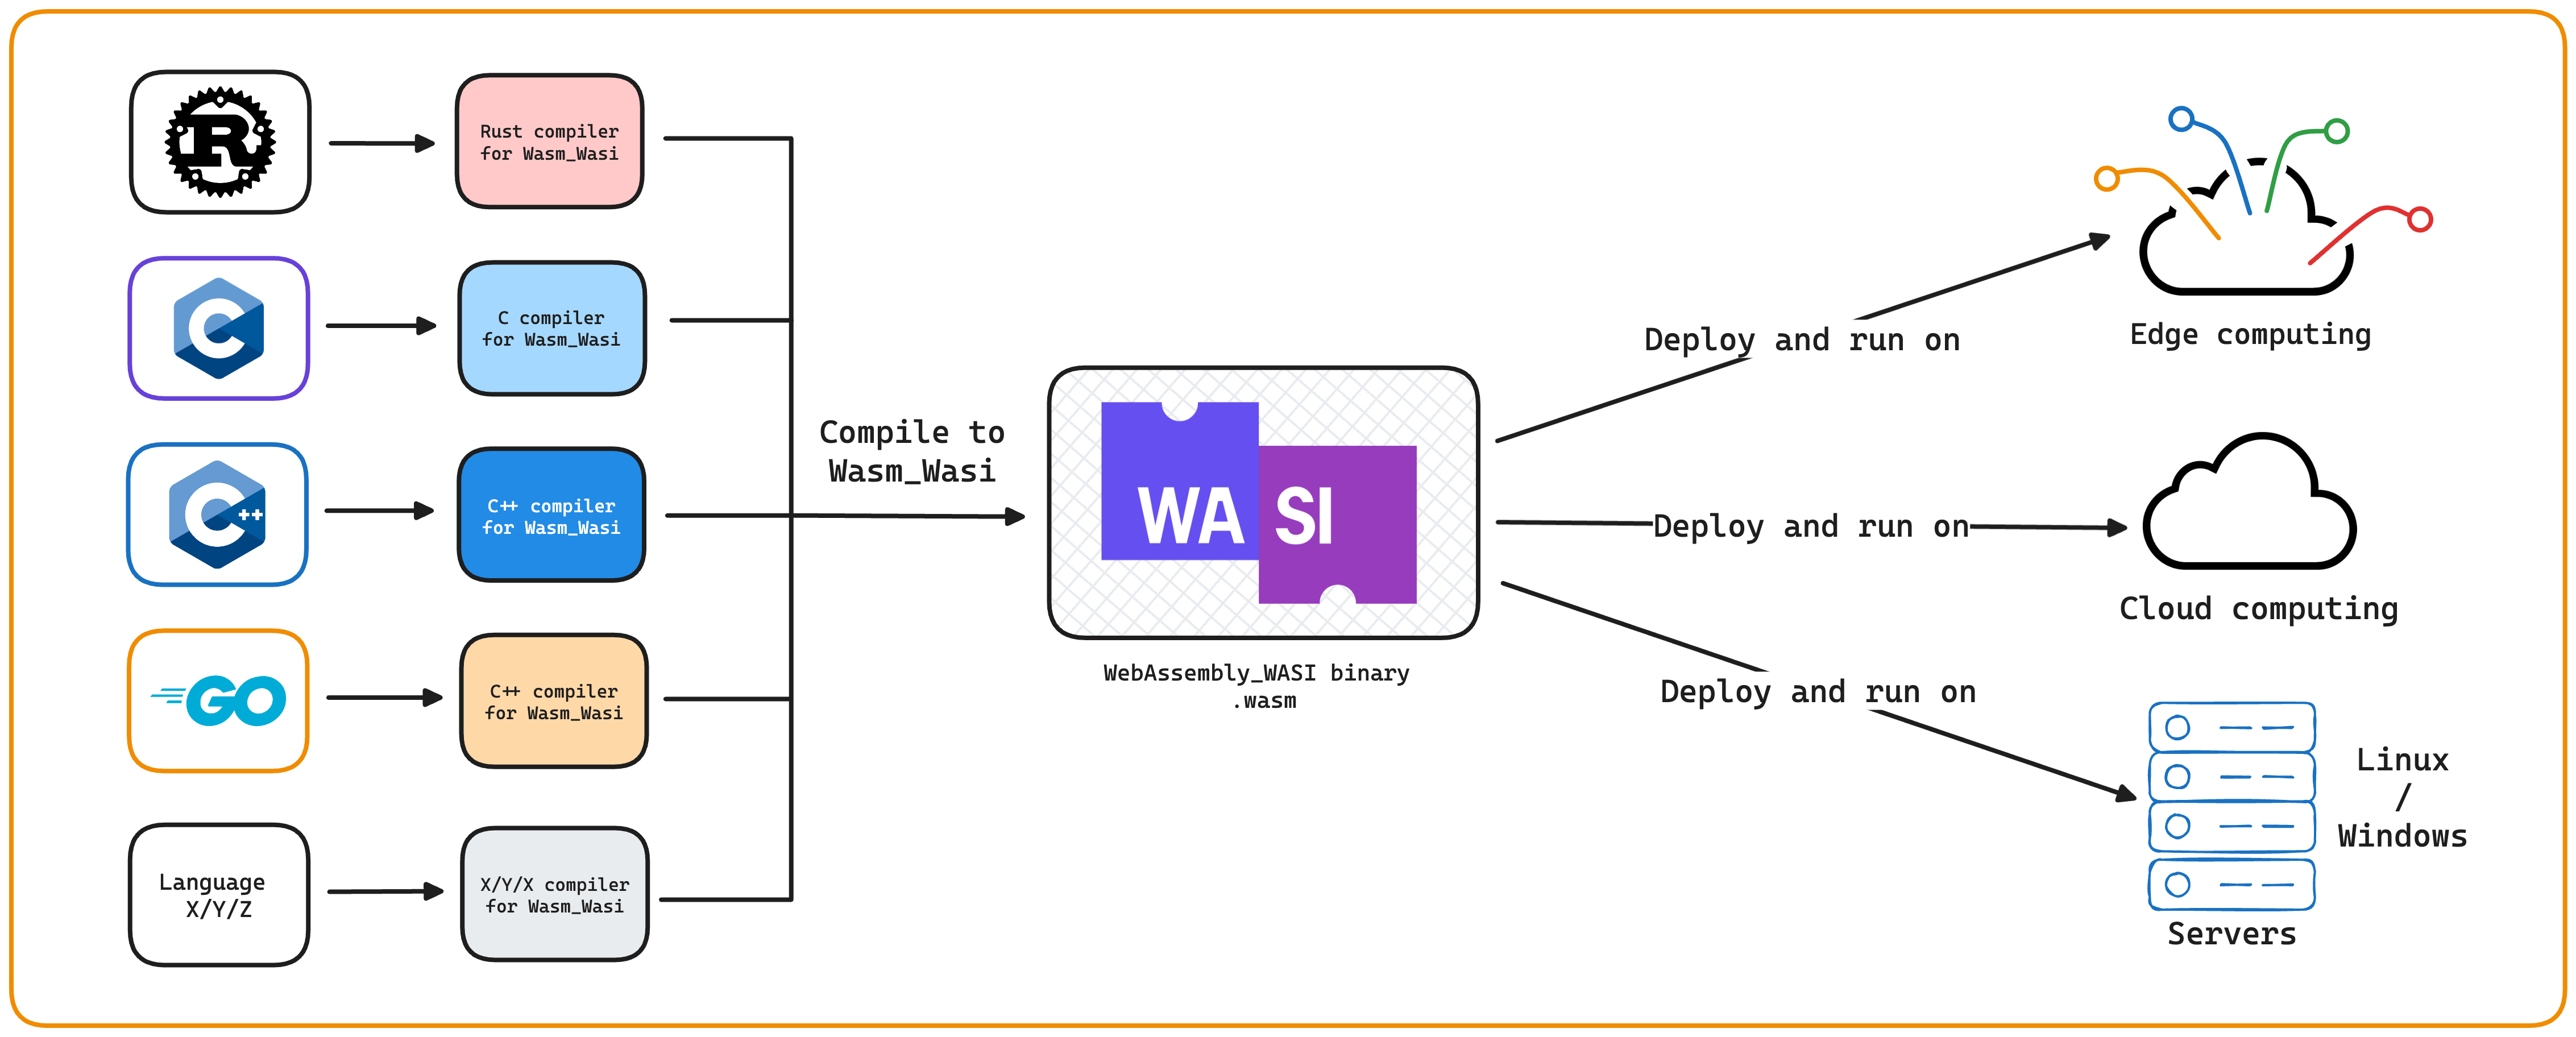
\includegraphics{assets/3-wasi-figure.png}
  \caption{Source code compiled to wasm\_wasi32 and deployed on platforms that support running the binaries.}
  \label{fig:wasm-wasi}
\end{figure}

\subsection{WebAssembly runtimes}

WebAssembly modules cannot run independently; they require a runtime
environment to interpret and execute them. Several WebAssembly runtimes
have been developed to support the execution of WebAssembly modules in
different environments, such as Wasmtime, Wasmer, and WasmEdge
\citep{zhang2024}.

\citet{zhang2024} explains that these runtimes provide a secure and
efficient execution environment for WebAssembly modules, enabling them
to run on a wide range of platforms, including cloud servers, edge
devices, and even embedded systems. They explain that some runtimes
offer features like \ac{AOT} compilation, which can further improve the
performance of WebAssembly modules. \Cref{fig:wasm-runtimes} below
illustrates how code written in a compatible source code can run on
multiple

\begin{figure}[H]
\centering
  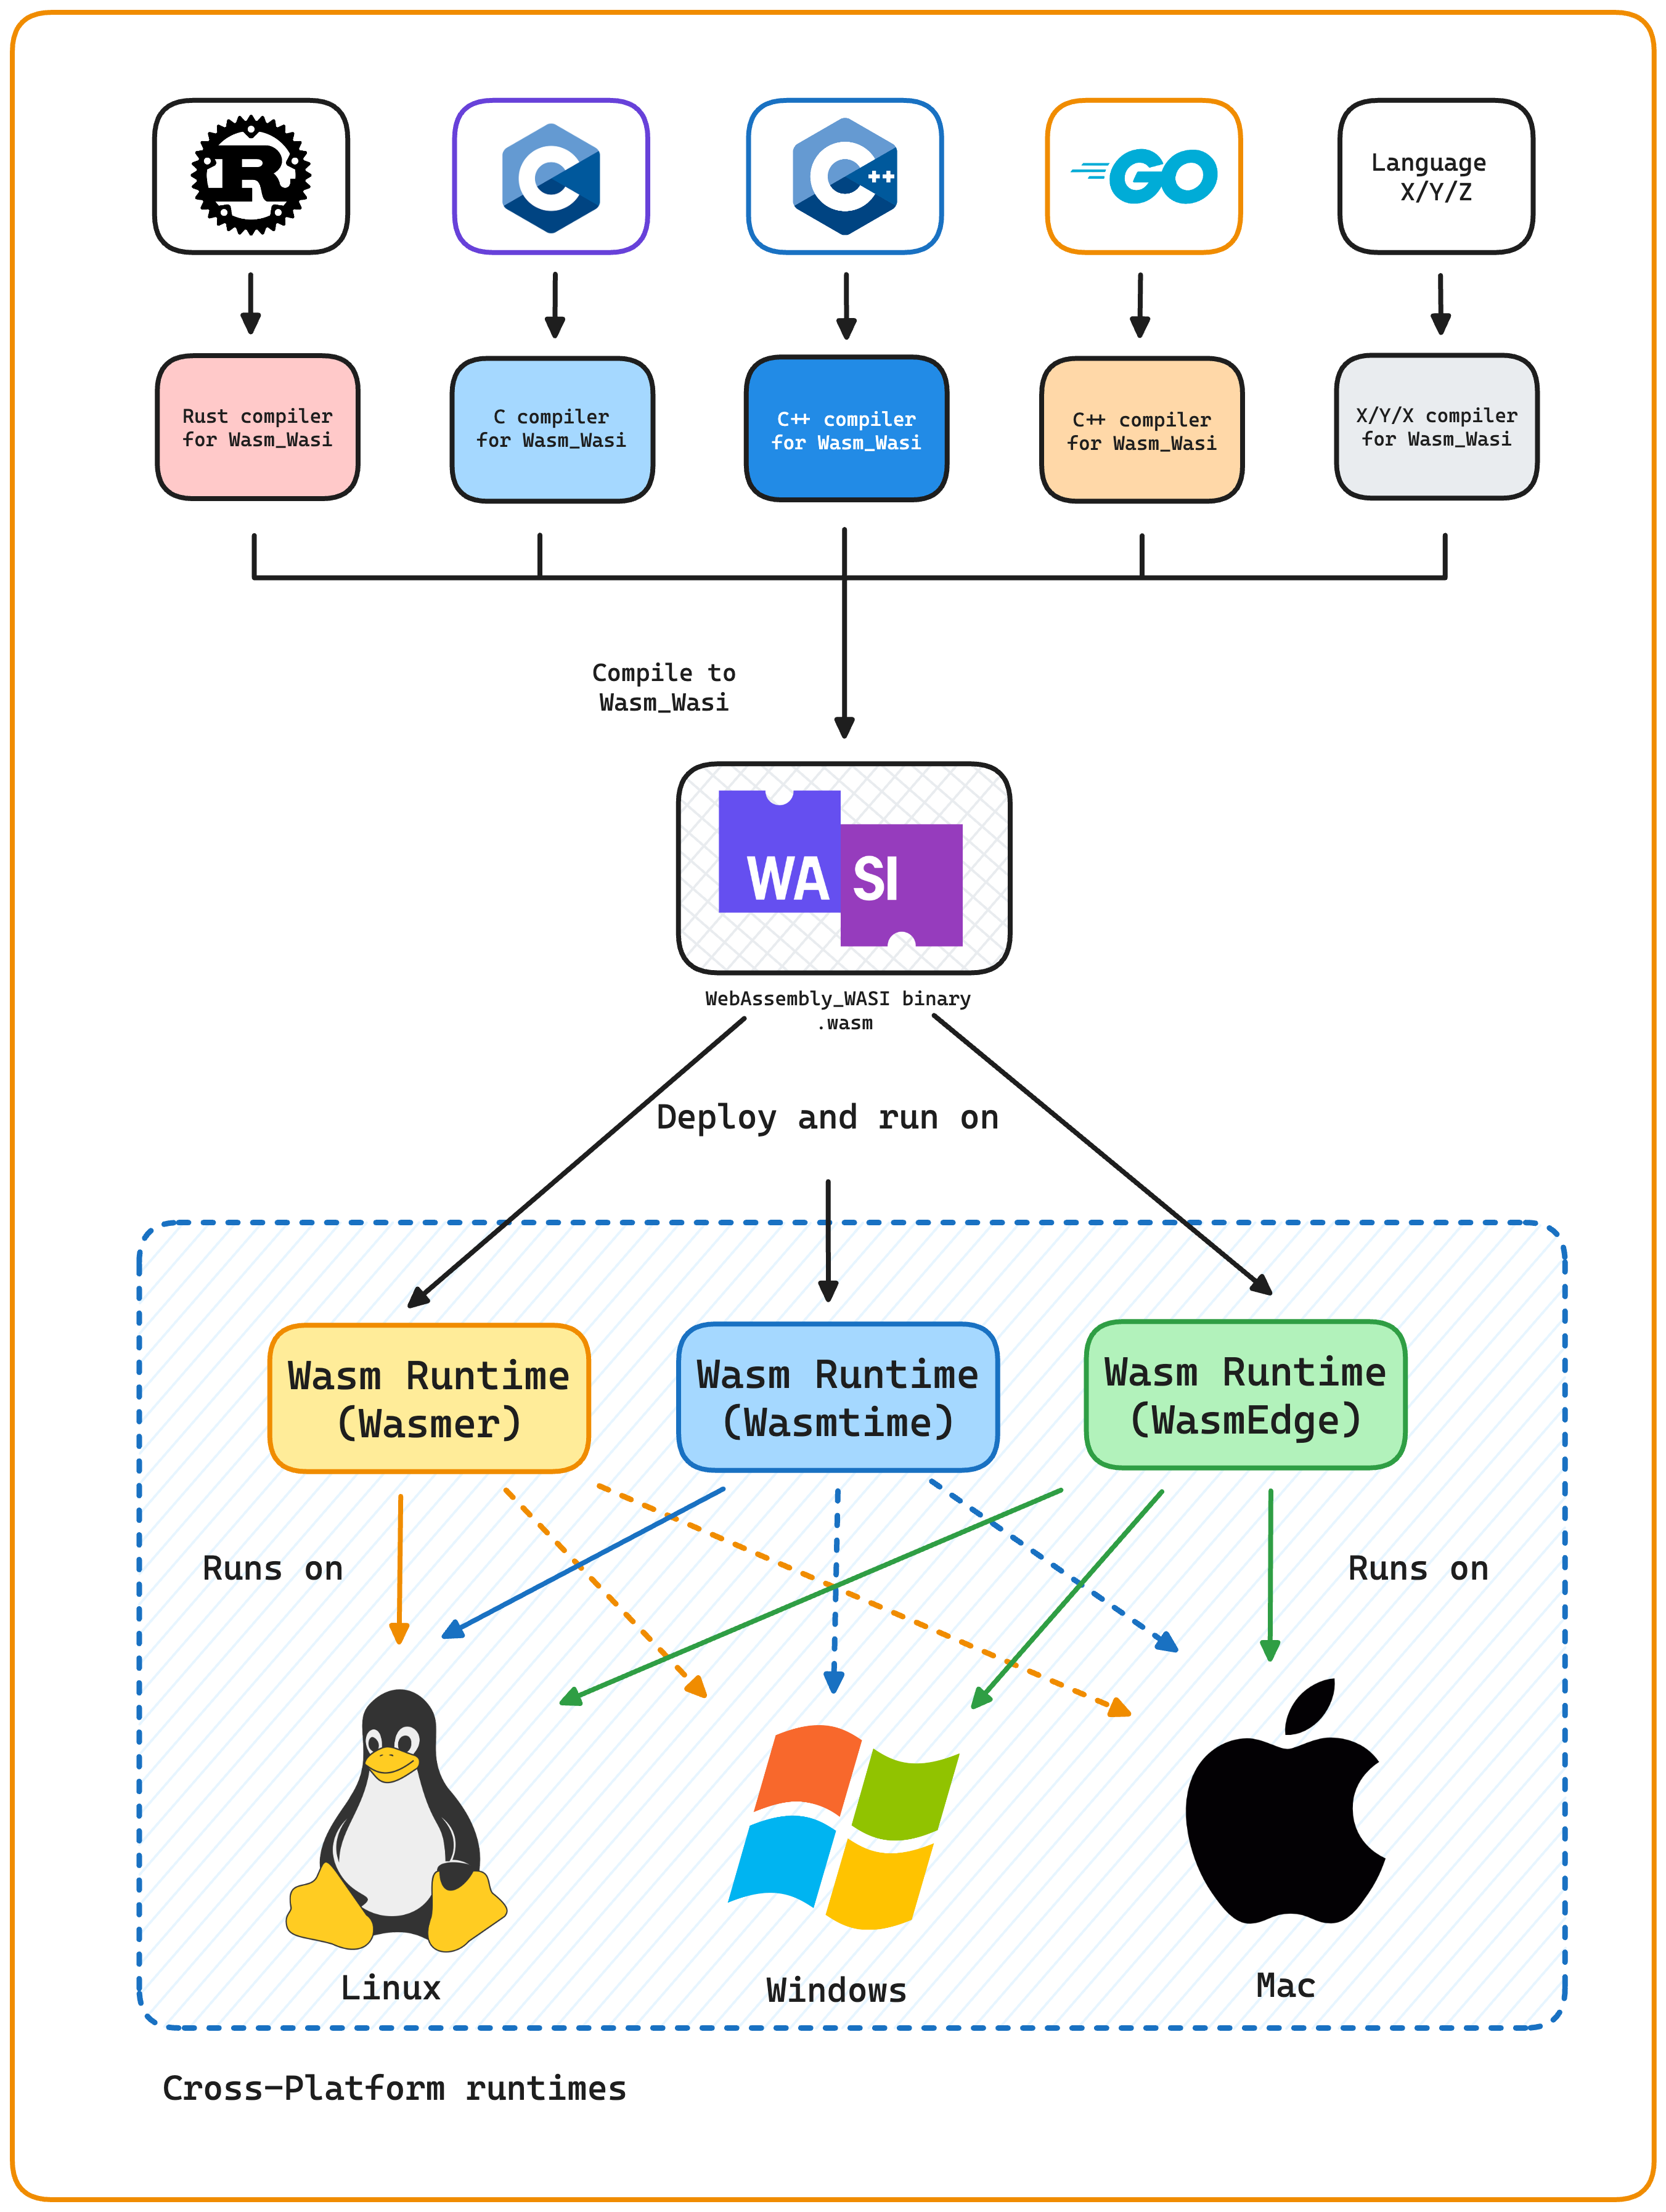
\includegraphics[width=0.7\columnwidth]{assets/3-wasm-runtime.png}
  \caption{Source code compiled to wasm\_wasi32 that can run anywhere
a WebAssembly runtime can be installed.}
  \label{fig:wasm-runtimes}
\end{figure}

The combination of WebAssembly, WASI, and efficient runtimes has sparked
interest in using WebAssembly as an alternative to traditional
containerization technologies, such as Docker, in cloud-native and
serverless environments \citep{shillakerFaasmLightweightIsolation2020a,
sebrechtsAdaptingKubernetesControllers2022}.

\section{Energy monitoring}

Monitoring and measuring energy consumption can be useful for
understanding and optimizing the energy efficiency of cloud computing
environments. Energy measurements provide insights into the impact of
different technologies, architectures, and workloads on overall energy
usage
\citep{shehabiUnitedStatesData2016, al-fuqahaInternetThingsSurvey2015}.

Several protocols and techniques have been explored to collect and
analyze energy consumption data, and this thesis will explore some of
these. These protocols enable the transmission of energy data, which can
be used for optimizing energy efficiency
\citep{al-fuqahaInternetThingsSurvey2015}.

\subsection{MQTT}

The \ac{MQTT} protocol is a lightweight and efficient protocol that has
been used for energy monitoring. In an MQTT setup, a broker server acts
as an intermediary, facilitating communication between devices and
servers. This enables efficient data exchange between publishers and
subscribers \citep{al-fuqahaInternetThingsSurvey2015}. (See
\Cref{fig:mqtt-model.png}).

\begin{figure}[H]
\centering
  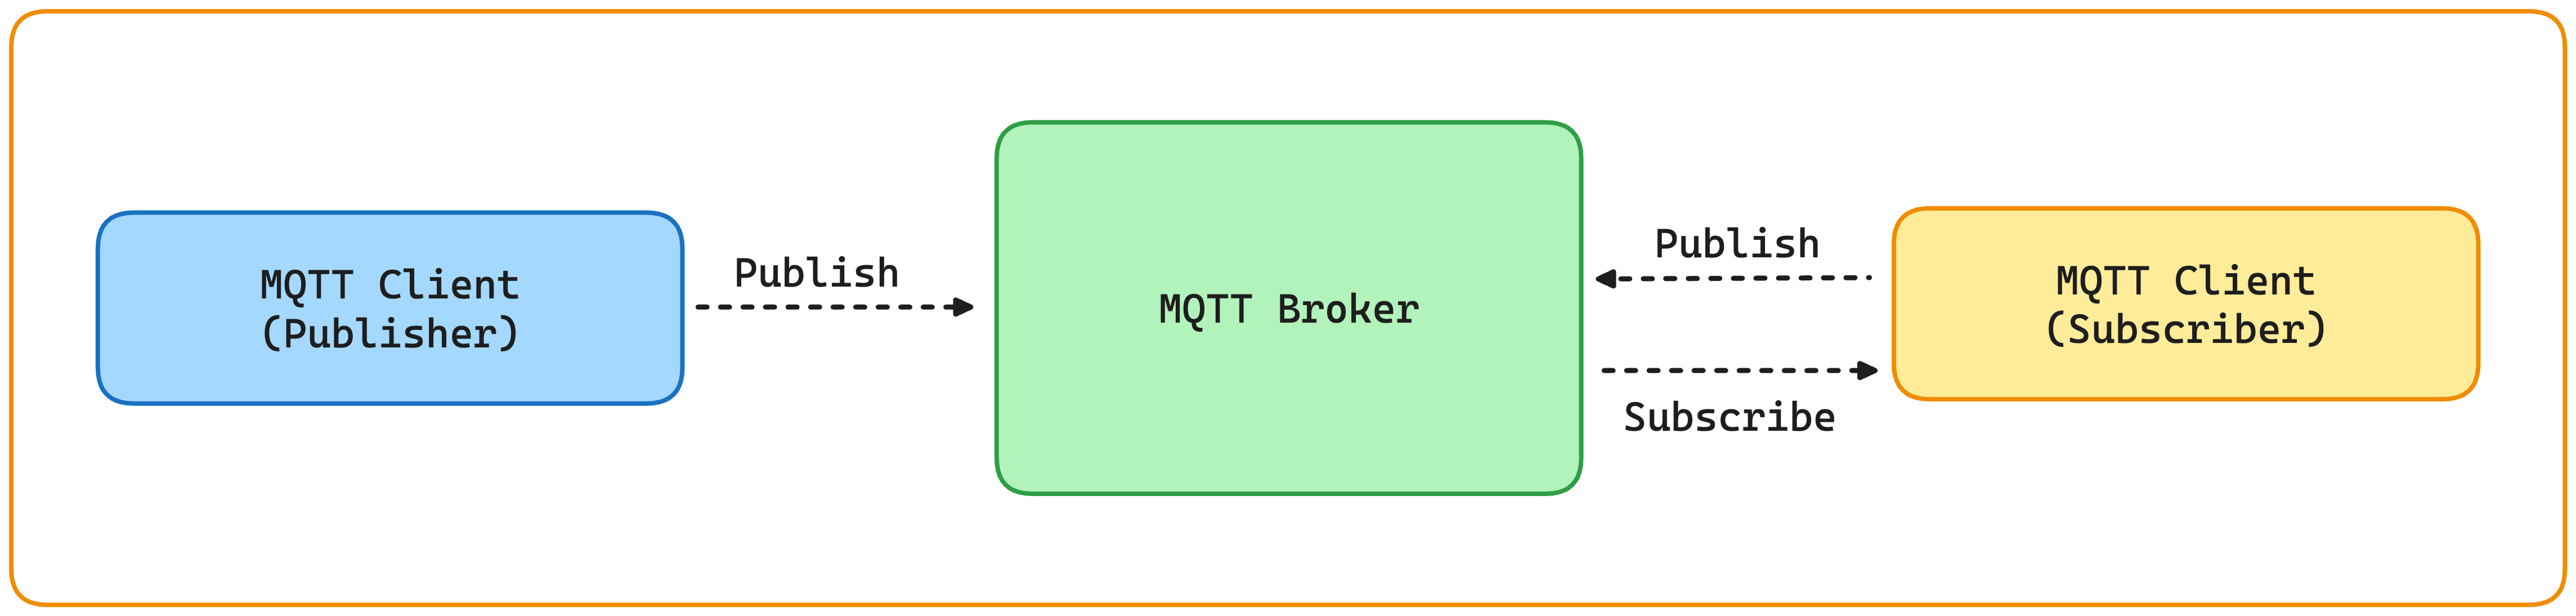
\includegraphics{assets/3-mqtt-pubsub.png}
  \caption{PubSub model of the MQTT protocol.}
  \label{fig:mqtt-model.png}
\end{figure}

\subsection{Z-Wave}

Z-Wave is a wireless communication protocol designed for home automation
and energy management. It has been used in research studies to develop
energy monitoring systems for residential buildings, enabling monitoring
and control of energy consumption
\citep{al-fuqahaInternetThingsSurvey2015}.

\todo{elaborate on why zwave is relevant. In the end, I ended up relying on
modbus because the latency the smart sockets supported were 1s at minimum}

\subsection{Modbus TCP}

The Modbus TCP protocol is a widely adopted industrial communication
protocol for exchanging data between devices and control systems. It has
been used to develop energy monitoring and auditing systems for
industrial applications, facilitating energy audits and energy-saving
strategies \citep{tongStudyEthernetCommunication2015}.

\part{Project}

\chapter{Methodology}

This chapter outlines the research methodology employed to investigate
the problem statements posed in \Cref{sect:problems}, specifically
whether \ac{Wasm} is a more energy-efficient target for developing and
deploying cloud native applications. A \ac{FaaS} prototype, named
`Nebula', will be developed as part of an experimental reserach method.
This prototype will be used to conduct experiments on startup latencies
(cold starts), runtime efficiency, and energy consumption of function
invocations in two different deployment environments: \ac{Wasm} modules
and Docker containers. The chapter details the research design,
experimental setup, data collection methods, and analysis techniques,
with a focus on ensuring the validity and reliability of the findings.

\section{Research design}

The objective of this thesis is to compare the performance and energy
efficiency of functions written in Rust when compiled to and deployed as
\ac{Wasm} modules versus the same functions compiled to a Rust binary
packaged in slim Docker containers. The research design will facilitate
an evaluation of these two environments for running functions in a
serverless model.

The research will be conducted through a series of controlled
experiments designed to measure startup latencies (cold starts), and
energy consumption under specified conditions. This experimental
approach allows for a for a precise evaluation of how \ac{Wasm}
technologies stack up against traiditional container-based deployments
in the context of cloud-native applications.

The experiments have beeen narrowed down to two domains:

\begin{enumerate}
\def\labelenumi{\arabic{enumi}.}
\item
  Deployment Environments: The choice of \ac{Wasm} modules and Docker
  containers as the primary environments for deployment is aimed at
  testing the core capabilities of \ac{Wasm} in a cloud-native setting,
  contrasting it against the well-established container technology. In a
  sense the experiments will compare two waves cloud compute.
\item
  Performance metrics: Metrics have been chosen to provide quantitative
  data on the efficiency and scalability of each technology. This
  includes measuring the time to initialize (cold start), the time to
  execute tasks (runtime), and the energy required for operations.
\end{enumerate}

\subsection{Sampling Strategy}

A total of four benchmark functions will be selected for testing,
representing various computational workloads. These functions will be
implemented in Rust and compiled to both \ac{Wasm} modules and Docker
images. The selection of these functions is based on computational
intensity and the ability to push the CPU, emulating real-world
scenarios.

The following sections will dive deeper into the specific methodologies
that will be employed for this thesis research.

\section{Experimental framework}

The main focus for this thesis is on building a prototype and perform
experiments on it, to measure the capabilities of \ac{Wasm}, augmented
by \ac{WASI} as a model for deploying and running cloud applications. An
experimental approach was chosen to test the problem statements posed in
\Cref{sect:problems}, as it allows for controlled manipulation of
variables, empirical measurements of outcomes, and direct comparison
between two deployment environments (\ac{Wasm}+\ac{WASI} and Docker).
This section outlines the different methods employed as part of an
experimental research method to investigate the research questions.

\subsection{Prototyping}

The prototype FaaS system, named `Nebula', will be developed to serve as
a controlled environment for invoking functions as either \ac{Wasm}
modules or Docker containers. It needs

To perform the desired experiments, a prototype will be developed and
deployed to two types of hardware. It will need to support invoking
functions compiled to \ac{Wasm} and functions packaged as Docker images.

\subsubsection{Hardware specifications}

Experiments will be performed on two types of hardware:

\begin{enumerate}
\def\labelenumi{\arabic{enumi}.}
\item
  Raspberry Pi: A small \ac{SBC}s with an ARM64 architecture that can
  run flavors of Linux. This device will be used to measure energy
  consumption relative to function invocations, which it is well suited
  for, as it consumes small amounts of energy by itself, making it ideal
  for comparing power consumption under actual load
  \citep{bekarooPowerConsumptionRaspberry2016}.
\item
  Virtual Machine: A Debian-based VM running on an \ac{IaaS} platform,
  to measure performance relative to what a standard cloud native
  application would perform.
\end{enumerate}

\subsubsection{Software specification}

\todo[inline=true]{Aknowledge that WASI allows for access to underlying system, but the
experiments will focus on running pure functions, which kinda diminishes
this point.}

For developing Nebula prototype itself, the following software setup
will be required:

\begin{itemize}
\tightlist
\item
  A programming language to write the prototype in.
\item
  An interface to deploy and invoke functions deployed onto the
  prototype.
\item
\end{itemize}

The software setup for developing functions will include:

\begin{itemize}
\tightlist
\item
  Rust programming language: Chosen for implementing functions due to
  its efficiency and compatibility when building with targeting both
  \ac{Wasm} and traditional binaries.
\item
  \ac{Wasm} and \ac{WASI}: The functions will be compiled as \ac{Wasm}
  binaries with the \texttt{wasm32-wasi} target when building with Rust.
\item
  Docker: Functions will also be packaged as Docker images for
  comparison purposes.
\end{itemize}

WASI allows for access to the underlying system, but the experiments
will focus on running pure functions, which doesn't allow this feature
to shine. The role of WASI is to provide a way to deploy and run
\ac{Wasm} modules in a cloud-native setting.

\subsection{Benchmarking}

Benchmarking will be employed as a research method to evaluate the
performance of different configurations. Benchmark functions
representing various computational workloads will be implemented and
executed on both environments.

\subsection{Empirical measurements}

Empirical measurement techniques will be utilized to quantify the energy
consumption associated with function invocations on each deployment
environment. The prototype and function binaries and images will be
deployed to the Raspberry Pi, which will be connected to a power supply
that can report energy readings.

\subsection{Controlled experimentation}

Controlled experimentation will be a crucial aspect of this research, as
it will allow for isolating and studying the effects of the deployment
environment on performance and energy consumption. Various factors, such
as input parameters for the benchmark functions and hardware
configurations, will be controlled or kept constant across experiments
to minimize the influence of external factors and ensure the validity
and reliability of the results.

\todo[inline=true]{elaborate that the functions chosen are to be Pure, meaning that Nebula in
its current state has been used a PFaaS (pure functions as a service)}

To experiment on Nebula, a handful of functions will be implemented,
which requires more computation as the input value scales up, to measure
exeuction time.

\subsubsection*{Fibonacci}

Find the \emph{nth} Fibonacci number in the sequence.

\[F_n = F_{n-1} + F_n \]

The Fibonacci sequence is a classic example of a recursive function. As
the input value (n) increases, the number of recursive calls grows
exponentially, leading to a significant increase in computation time.
This makes it an excellent candidate for testing the performance of your
prototype under increasing computational load.

\subsubsection*{Exponential}

Calculate the value of Euler's number raised to the \emph{nth} power.

\[F_n = e^n \]

\subsubsection*{Factorial}

Calculate the sum of the factorial of \emph{n}.

\[ n! = \prod_{k=1}^n k \]

\subsubsection*{Prime number}

Find the \emph{nth} prime number. While this function is harder to
represent mathematically, and while Euler deduced a close approximation
with \(P(n) = n^2 - n +
41\), a function will be written in a more brute-force manner to push
the CPU, and emulate a more typical scenario.

This function will be expressed with these constraints:

\[ \text{is\_prime}(n) =
\begin{cases} 
\text{false} & \text{if } n \leq 1 \\
\text{true} & \text{if } n = 2 \text{ or } n = 3 \\
\text{false} & \text{if } n \mod 2 = 0 \text{ or } n \mod 3 = 0 \\
\text{false} & \text{if } \exists k, \text{ such that } 5 \leq k \leq \sqrt{n}, k \in \{6i-1, 6i+1\}, n \mod k = 0 \\
\text{true} & \text{otherwise}
\end{cases}
\]

And with a loop that ranges from 1 to \(2^{64} - 1\) (the highest
integer on the target architecture), check if that number is prime, if
so, append it to a list of primes and check if the new length of the
list equals the input \emph{n}.

\subsection{Comparative analysis}

A comparative anlysis will be performed to evaluate the cold starts,
runtime, and the energy consumption of function invocations between the
two deployment environments. Specific metrics, such as startup latency,
execution time, and energy consumption per invocation, will be used for
this comparison to assess the overall performance and energy efficiency
of each deployment environment for serverless function execution.

\subsection{Data collection and analysis}

Throughout the experiments, various data points, including startup and
execution times, and energy consumption readings, will be collected and
stored. Statistical techniques, such as mean, median, and standard
deviation calculations, will be employed to analyze the collected data.
Aditionally, regression analysis will be used to model the relationship
between the independent variables (deploymend environment and function
type) and the dependent variables (startup latency, execution time, and
energy consumption). o

\subsection{Reliability and Validity}

To ensure the reliability and validity of the results, the following
measures will be taken: controlled experimentation will be used to
minimize the influence of external factors; the experiments will be
repeared multiple times to ensure consistency of the results; the data
will be analyzed using statistical techniques to identify any patterns
or trends; and the results will be validated by comparing them to
existing research in the field, explored in \Cref{sect:related-work}.

\begin{verbatim}
Marius thoughts:

Some aspects of cloud-native applications, like "impure" functionality is
discounted for this research. The functions don't read to/fro the underlying
system or perform intensive I/O operations. This is to compare functions in more
of a controlled and isolated manner, where the time it takes to invoke a
function in wasm focuses on the calculation itself. This is also true for the
Docker images, so it's still a fair assessment. 
\end{verbatim}

\chapter{Designing Nebula}

This chapter will present the design and overall architecture of Nebula,
a \ac{FaaS} prototype that can spin up functions both as \ac{Wasm}
modules, and as Docker images. The core components of the prototype will
be presented, and by the end of this chapter, the reader should have a
clear understanding on how Nebula was designed, how its core features
were chosen for implementation and how one can interact with the
prototype.

\section{A word on this chapter}

This is a prototype FaaS platform that is meant to illustrate the raw
differences between two waves of cloud compute; \ac{Wasm} modules and
container. It's scope will be limited by the fact that it is a single
students thesis project, and will naturlly lack many features that
large-scale FaaS platforms typically have. None of the major cloud
providers have open sourced their FaaS platform, meaning that exactly
how they function behind the scenes is difficult to surmise. This
prototype therefore aims to hone in on the aspect of deploying functions
as containers and compare it with deploying functions as \ac{Wasm}
modules.

\section{Nebula overview}

\todo[inline=true]{

This section will provide an overview of Nebula's architecture, including: 

- A high-level description of the system components and their relationship.
- An explanation of how users can interact with Nebula.
- A brief discussion of the design trade-offs made during development.

}

\section{Core components}

The following sections will delve into the individual core components of
Nebula:

\subsection{Web server}

\subsection{Function deployment}

How functions are packaged, deployed and managed on the server.

\subsection{Wasm Module execution}

\todo[inline=true]{The process by which \ac{Wasm} modules are executed on Nebula.}

\subsection{Docker Image execution}

\todo[inline=true]{The process by which Docker images are executed on Nebula.}

\subsection{Orchestration and Management}

\todo[inline=true]{How Nebula manages the execution of functions, including passing input/output
and collecting metrics}

\section{Design rationale}

\todo[inline=true]{Explain that this section provide an explanation of design decisions made
during development of Nebula}

\section{Designing energy readings}

\newpage

\chapter{Implementing Nebula}

This chapter provides the details of the implementation of Nebula.

\section{Requirements}

\newpage

\part{Results}

\newpage
\chapter{Evaulation}

\newpage
\chapter{Discussion}

\section{Related work}
\label{sect:related-work}

\todo[inline=true]{Maybe this section should be moved to the discussion/results page and be
pulled in to support my findings?}

There are several cloud providers who have added support for running
\ac{Wasm} on their cloud offerings. Cloudflare Workers\footnote{\url{https://developers.cloudflare.com/workers/runtime-apis/webassembly/}},
and Fastly
\href{mailto:Compute@Edge}{\nolinkurl{Compute@Edge}}\footnote{\url{https://www.fastly.com/products/edge-compute/serverless}}
have added support, while Fermyon have built an entire cloud
architecture around the binary format with their Fermyon
Cloud\footnote{\url{https://www.fermyon.com/cloud}}. Fermyon has also
open sourced their developer tool Spin\footnote{\url{https://www.fermyon.com/spin}},
a tool that lets developers create, build and test applications written
in a supported language\footnote{\url{https://developer.fermyon.com/spin/v2/language-support-overview}}
and deploy it to a Fermyon Platform instance, either self-hosted or on
their own service.

\citet{sebrechtsAdaptingKubernetesControllers2022} wrote a paper where
they described their research in developing a \ac{Wasm}-based framework
for running lightweight controllers on Kubernetes. In their research
they found that with their novel \ac{Wasm}-based operators were able to
reduce memory footprint of 100 synthetic operators from 1405MiB to
227MiB and from 1131MiB to 86MiB of idle operators, compared to
traditional operators. One of their conclusions is that using \ac{Wasm}
proved to be more memory efficient than the container-based solution.
See \Cref{fig:wasm-memory} for their findings on memory usage with
\ac{Wasm}-based operators to Rust and Golang operators.

\begin{figure}[H]
\centering
  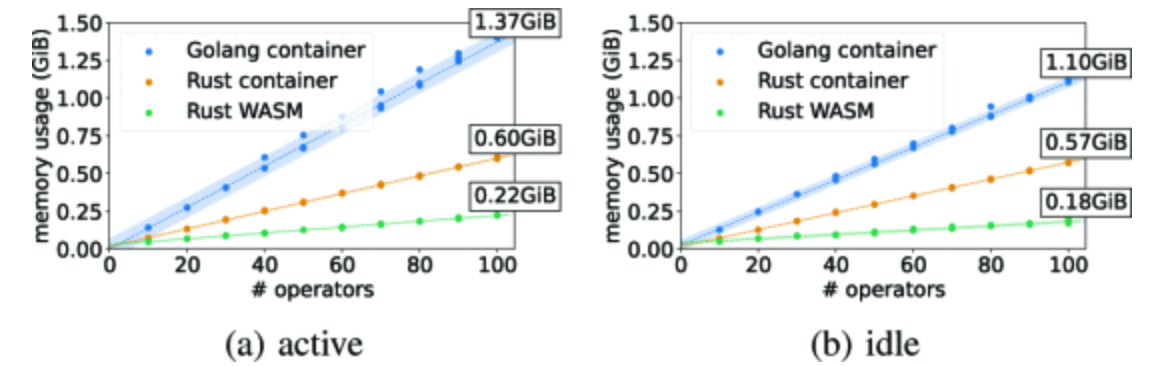
\includegraphics{assets/3.8-memoryusage-wasm.png}
  \caption{Different Kubernetes operators memory usage. Comparing Rust to WASM
vs Rust container vs Golang container. © 2022 IEEE}
  \label{fig:wasm-memory}
\end{figure}

\citet{shillakerFaasmLightweightIsolation2020a} introduced a novel
serverless runtime framework using an abstraction called Faaslets, which
employ \ac{Wasm} for software-fault isolation (SFI). Their study showed
that Faaslets in the Faasm runtime significantly enhance performance and
efficiency over traditional container-based platforms. Notably, they
achieved 2x speed-up in machine learning model training and doubled the
throughput for interference tasks, while reducing memory usage by 90\%,
compared to traditional containers with Knative. See
\cref{fig:wasm-faasm} below for their findings while comparing their
Faasm to Knative.

\begin{figure}[H]
\centering
  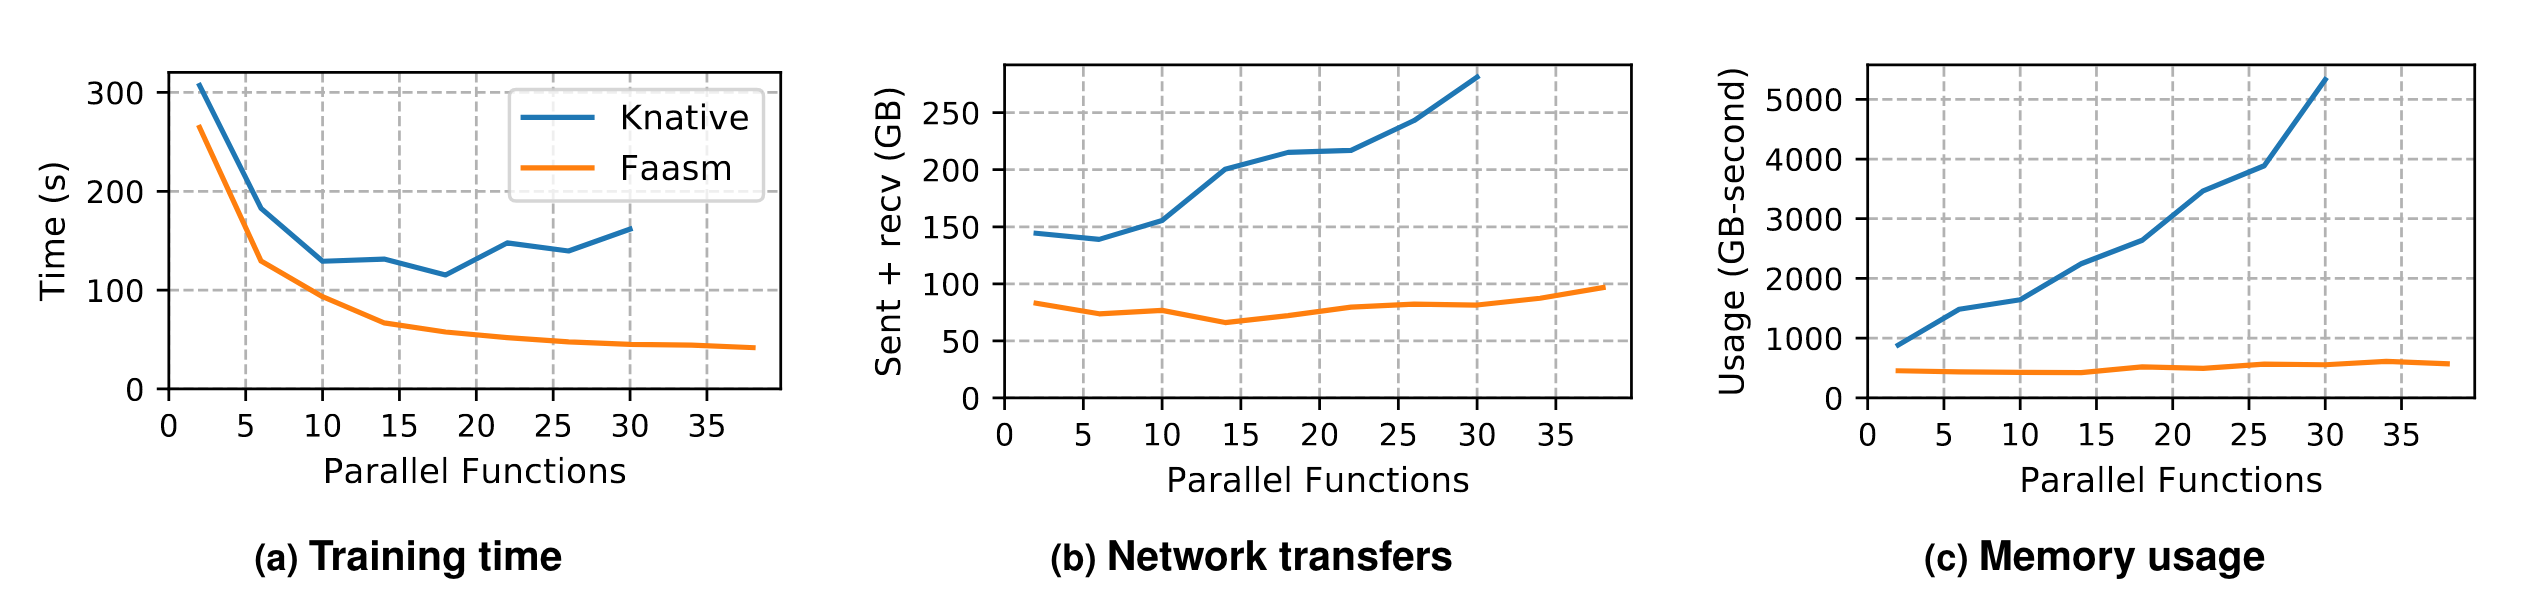
\includegraphics{assets/3.8-faasm.png}
  \caption{Different Kubernetes operators memory usage. Comparing Rust to WASM
vs Rust container vs Golang container. © 2022 IEEE}
  \label{fig:wasm-faasm}
\end{figure}

Furthermore, \citet{shillakerFaasmLightweightIsolation2020a} documented
the details of the cold starts they observed during their experiments.
In their study they found that cold starts for operators based on
\ac{Wasm} were 538 times faster than the traditional container-based
operators and occupied between 6.5 to 25 times less memory while in
operation. See \Cref{tab:dockervsfaaslet} below for their findings.

\begin{table}[H]
\centering
\caption{\label{tab:unnamed-chunk-1}The table is here \label{tab:dockervsfaaslet}}
\centering
\begin{tabu} to \linewidth {>{\raggedright}X>{\raggedleft}X>{\raggedleft}X>{\raggedleft}X}
\toprule
 & Docker & Faaslets & vs.Docker\\
\midrule
\cellcolor{gray!10}{Initialization} & \cellcolor{gray!10}{2.8 s} & \cellcolor{gray!10}{5.2 ms} & \cellcolor{gray!10}{538×}\\
CPU cycles & 251M & 1.4K & 179K×\\
\cellcolor{gray!10}{PSS memory} & \cellcolor{gray!10}{1.3 MB} & \cellcolor{gray!10}{200 KB} & \cellcolor{gray!10}{6.5×}\\
RSS memory & 5.0 MB & 200 KB & 25×\\
\cellcolor{gray!10}{Capacity} & \cellcolor{gray!10}{\textasciitilde{}8 K} & \cellcolor{gray!10}{\textasciitilde{}70 K} & \cellcolor{gray!10}{8×}\\
\bottomrule
\end{tabu}
\end{table}

\newpage
\chapter{Conclusion}

\newpage
\chapter{Future work}

\chapter*{Acronyms}
\begin{acronym}
  \acro{IaaS}[IaaS]{Infrastructure-as-a-Service}
  \acro{FaaS}[FaaS]{Functions-as-a-Service}
  \acro{Wasm}[Wasm]{WebAssembly}
  \acro{WASI}[WASI]{WebAssembly System Interface}
  \acro{VMs}[VMs]{virtual machines}
  \acro{VM}[VM]{virtual machine}
  \acro{JVM}[VM]{Java Virtual Machine}
  \acro{NIST}[NIST]{National Institute of Standards and Technology}
  \acro{AWS}[AWS]{Amazon Web Services}
  \acro{GCP}[GCP]{Google Cloud Platform}
  \acro{ACI}[ACI]{Azure Container Instances}
  \acro{SBC}[SBC]{Single board computer}
  \acro{AOT}[AOT]{ahead-of-time}
  \acro{MQTT}[MQTT]{Message Queuing Telemetry Transport}
\end{acronym}

\chapter*{Appendices}

\printbibliography

\end{document}
